\documentclass[aspectratio=169]{beamer}

\setbeamertemplate{navigation symbols}{}
\usetheme{Boadilla}
\usepackage[italian]{babel}
\usepackage[dvipsnames]{xcolor}
\usepackage{minted}
\usepackage{calc} 

\title{Gestione Documenti - Versione Pure-HTML}
\author{Lorenzo Chiroli (C.P. 10797603 - MTR. 981392)}
\date{Gruppo N. 120}

\begin{document}
\frame{\titlepage}

\begin{frame}
    \frametitle{Specification and Optional Additions - 1}
    L’applicazione supporta registrazione e login mediante una pagina pubblica con opportune form. La registrazione
    richiede l’inserimento di username, indirizzo di email e password e controlla la validità sintattica dell’indirizzo
    di email e l’uguaglianza tra i campi “password” e “ripeti password”. La registrazione controlla l’unicità dello
    username. \newline

    \textit{Viene assunto che sia lecito per un utente registrarsi K volte all'applicazione utilizzando la medesima
        e-mail a condizione che venga rispettata l'univocità dell'username.} \newline

    Una cartella ha un proprietario, un nome e una data di creazione e può contenere altre cartelle e/o documenti. Un
    documento ha un proprietario, nome, una data di creazione, un sommario e un tipo. Quando l’utente accede
    all’applicazione appare una HOME PAGE che contiene un albero delle proprie cartelle e delle sottocartelle.
\end{frame}

\begin{frame}
    \frametitle{Specification and Optional Additions - 2}
    Nell’HOME PAGE l’utente può selezionare una cartella e accedere a una pagina CONTENUTI che mostra l’elenco delle
    cartelle e dei documenti di una cartella. Ogni documento in elenco ha due link: \underline{accedi} e
    \underline{sposta}.

    \begin{itemize}
        \item Quando l’utente seleziona il link \underline{accedi}, appare una pagina DOCUMENTO (nella stessa finestra
              e tab del browser) che mostra tutti i dati del documento selezionato.
        \item Quando l’utente seleziona il link \underline{sposta}, appare la HOME PAGE con l’albero delle cartelle; in
              questo caso la pagina mostra il messaggio “Stai spostando il documento X dalla cartella Y. Scegli la
              cartella di destinazione”, la cartella a cui appartiene il documento da spostare NON è selezionabile e il
              suo nome è evidenziato (per esempio con un colore diverso). Quando l’utente seleziona la cartella di
              destinazione, il documento è spostato dalla cartella di origine a quella di destinazione e appare la
              pagina CONTENUTI che mostra il contenuto aggiornato della cartella di destinazione.
    \end{itemize}
\end{frame}

\begin{frame}
    \frametitle{Specification and Optional Additions - 3}
    Ogni pagina, tranne la HOME PAGE, contiene un collegamento per tornare alla pagina precedente. L’applicazione
    consente il logout dell’utente da qualsiasi pagina. \newline

    \textit{Viene inoltre aggiunto, nelle pagine diverse dalla HOME PAGE, un link per tornare alla pagina principale.
        Il collegamento per tornare alla pagina precedente, nella pagina "CONTENUTI" è implementato in modo da seguire
        la directory structure creata dall'utente.} \newline

    Una pagina GESTIONE CONTENUTI raggiungibile dalla HOME PAGE permette all’utente di creare una cartella di primo
    livello, una cartella all’interno di una cartella esistente e un documento all’interno di una cartella.
    L’applicazione non richiede la gestione dell’upload dei documenti.
\end{frame}

\begin{frame}
    \frametitle{Data Requirements Analysis}
    [...] La registrazione [di un \textcolor{Red}{utente} N.d.R.] richiede l’inserimento di
    \textcolor{Green}{username}, \textcolor{Green}{indirizzo di email} e \textcolor{Green}{password} e controlla la
    validità sintattica dell’indirizzo di email e l’uguaglianza tra i campi “password” e “ripeti password”. La
    registrazione controlla l’unicità dello username. \newline

    Una \textcolor{Red}{cartella} \textcolor{Blue}{ha un} \textcolor{Red}{proprietario} [a.k.a. un
        \textcolor{Red}{utente} N.d.R.], un \textcolor{Green}{nome} e una \textcolor{Green}{data di creazione} e
    \textcolor{Blue}{può contenere altre} \textcolor{Red}{cartelle} e/o \textcolor{Red}{documenti}. Un
    \textcolor{Red}{documento} \textcolor{Blue}{ha un} \textcolor{Red}{proprietario}, \textcolor{Green}{nome}, una
    \textcolor{Green}{data di creazione}, un \textcolor{Green}{sommario} e un \textcolor{Green}{tipo}.
    [...]\footnotemark{}

    \footnotetext{I colori hanno il seguente significato: \textcolor{Red}{entità}, \textcolor{Green}{attributi}, e
        \textcolor{Blue}{relazioni}.}
\end{frame}

\begin{frame}
    \frametitle{Database Design}
    \begin{figure}
        \centering
        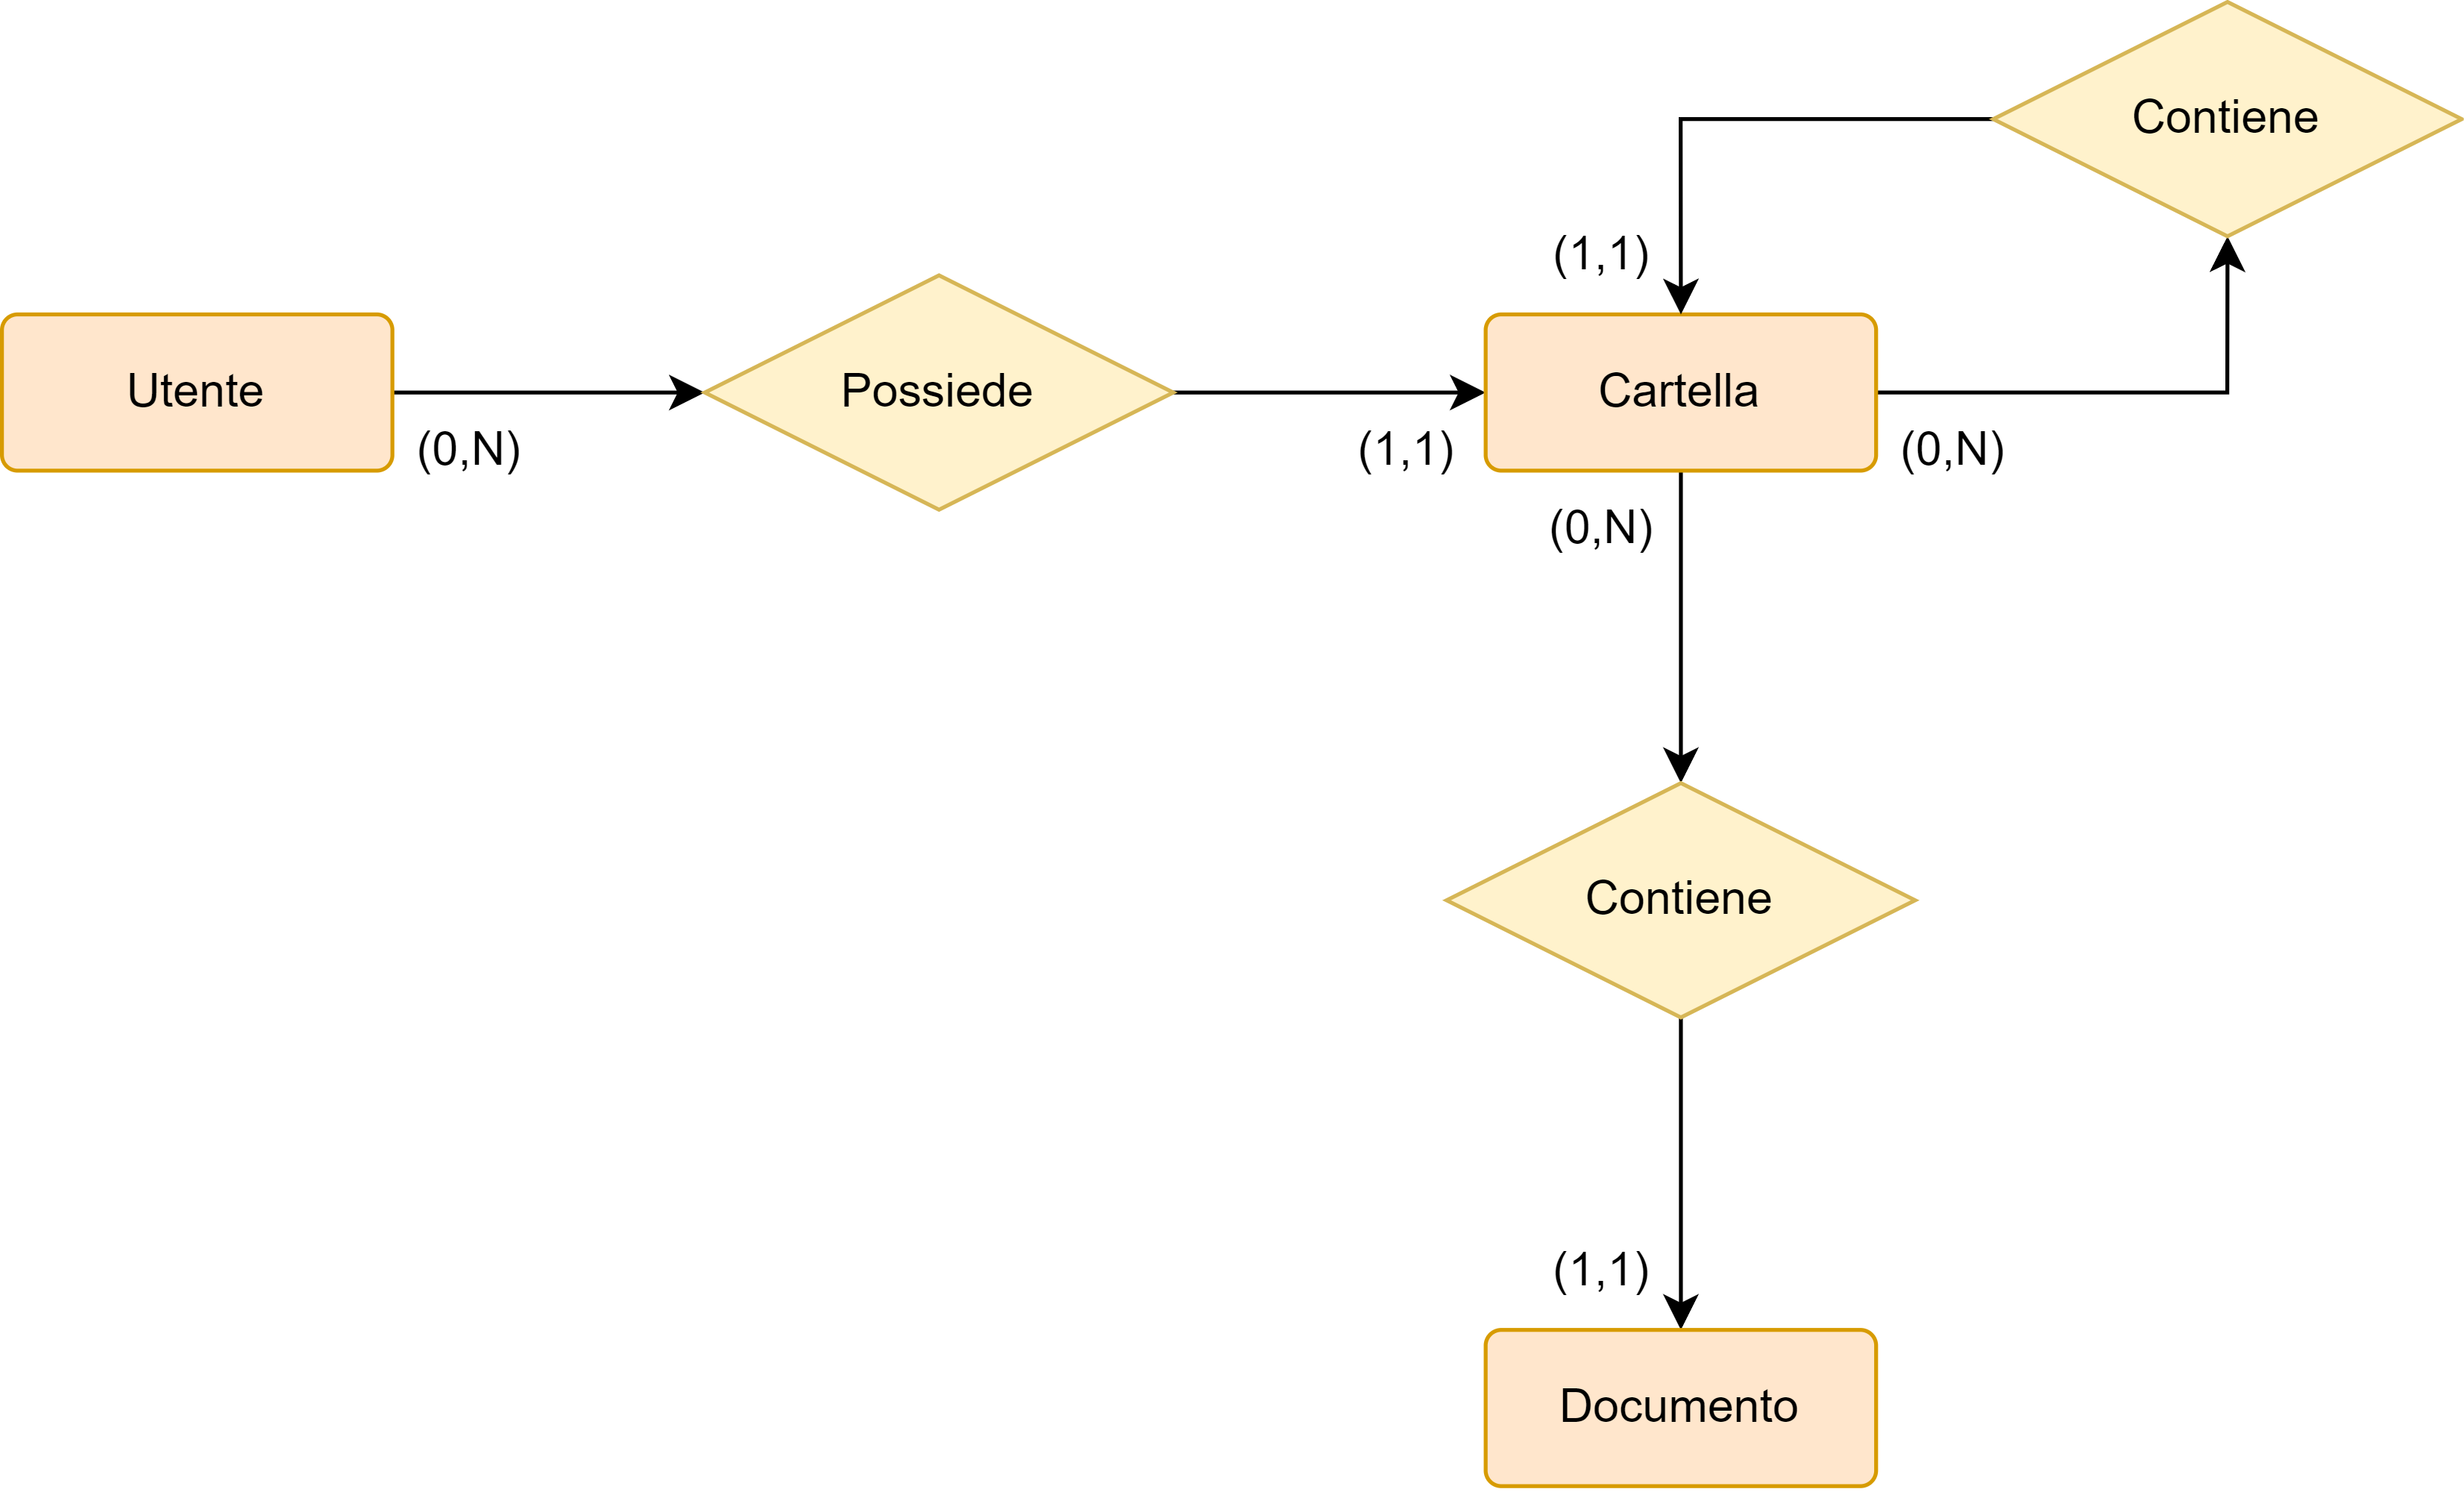
\includegraphics[width=0.75\linewidth]{Resources/ER-Diagram.png}
    \end{figure}
\end{frame}

\begin{frame}[fragile]
    \frametitle{Database Schema - 1}
    \scriptsize
    \begin{minted}{SQL}
CREATE TABLE IF NOT EXISTS Users
(
    UserID       INT AUTO_INCREMENT PRIMARY KEY, -- Unique identifier for each user
    Username     VARCHAR(64) UNIQUE NOT NULL,    -- User's chosen username, must be unique
    PasswordHash VARCHAR(128)       NOT NULL,    -- Hash of the user's password for security
    Email        VARCHAR(64)        NOT NULL     -- User's email address, must be unique
);
\end{minted}

    \rule{\textwidth}{0.5pt}

    \begin{minted}{SQL}
CREATE TABLE IF NOT EXISTS Folders
(
    FolderID       INT AUTO_INCREMENT PRIMARY KEY, -- Unique identifier for each folder
    FolderName     VARCHAR(64) NOT NULL,           -- Name of the folder
    CreationDate   DATETIME    NOT NULL,           -- Date and time the folder was created
    OwnerID        INT         NOT NULL,           -- UserID of the folder's owner
    ParentFolderID INT,                            -- FolderID of the parent folder, if any
    FOREIGN KEY (OwnerID) REFERENCES Users (UserID) ON DELETE CASCADE ON UPDATE CASCADE,
    FOREIGN KEY (ParentFolderID) REFERENCES Folders (FolderID) ON DELETE CASCADE ON UPDATE CASCADE
);
\end{minted}
\end{frame}

\begin{frame}[fragile]
    \frametitle{Database Schema - 2}
    \scriptsize
    \begin{minted}{SQL}
CREATE TABLE IF NOT EXISTS Documents
(
    DocumentID   INT AUTO_INCREMENT PRIMARY KEY, -- Unique identifier for each document
    DocumentName VARCHAR(64) NOT NULL,           -- Name of the document
    CreationDate DATETIME    NOT NULL,           -- Date and time the document was created
    Type         VARCHAR(64) NOT NULL,           -- Type of the document (e.g., PDF, TXT)
    Summary      VARCHAR(256),                   -- Optional summary of the document's content
    OwnerID      INT         NOT NULL,           -- UserID of the document's owner
    FolderID     INT,                            -- FolderID of the folder containing the document
    FOREIGN KEY (OwnerID) REFERENCES Users (UserID) ON DELETE CASCADE ON UPDATE CASCADE,
    FOREIGN KEY (FolderID) REFERENCES Folders (FolderID) ON DELETE CASCADE ON UPDATE CASCADE
);
\end{minted}
\end{frame}

\begin{frame}
    \frametitle{Application Requirements Analysis - 1}
    L’applicazione supporta \textcolor{Blue}{registrazione} e \textcolor{Blue}{login} mediante una
    \underline{pagina pubblica} [rif. a \textcolor{Red}{registrazione (UserRegistration)} e
        \textcolor{Red}{login (UserAuthentication)} N.d.R.] con \textcolor{Green}{opportune form}.
    La registrazione richiede l’inserimento di \textcolor{Green}{username}, \textcolor{Green}{indirizzo di email} e
    \textcolor{Green}{password} [e anche di \textcolor{Green}{"ripeti password"} N.d.R.; rif. "opportune form"] e
    \textcolor{Orange}{controlla la validità sintattica dell’indirizzo di email e l’uguaglianza tra i campi “password”
        e “ripeti password”}. La registrazione \textcolor{Orange}{controlla l’unicità dello username}. \newline

    Una cartella ha un proprietario, un nome e una data di creazione e può contenere altre cartelle e/o documenti. Un
    documento ha un proprietario, nome, una data di creazione, un sommario e un tipo.
    Quando l’utente \textcolor{Blue}{accede} all’applicazione \textcolor{Orange}{appare} una
    \textcolor{Red}{HOME PAGE (Homepage)} che contiene un \textcolor{Green}{albero delle proprie cartelle e delle
        sottocartelle}.\footnotemark{}

    \footnotetext{I colori hanno il seguente significato: \textcolor{Red}{pagine},
        \textcolor{Green}{componenti di visualizzazione}, \textcolor{Blue}{eventi} e \textcolor{Orange}{azioni}.}
\end{frame}

\begin{frame}
    \frametitle{Application Requirements Analysis - 2}
    Nell’\textcolor{Red}{HOME PAGE} l’utente può \textcolor{Blue}{selezionare una cartella} e
    \textcolor{Orange}{accedere} a una pagina \textcolor{Red}{CONTENUTI (ViewFolderContent)} che mostra
    \textcolor{Green}{l’elenco delle cartelle e dei documenti di una cartella}. Ogni documento in elenco ha due
    \textcolor{Green}{link: \underline{accedi} e \underline{sposta}}.\footnotemark{}

    \begin{itemize}
        \item Quando l’utente \textcolor{Blue}{seleziona il link \underline{accedi}}, \textcolor{Orange}{appare} una
              pagina \textcolor{Red}{DOCUMENTO (ViewDocumentDetails)} (nella stessa finestra e tab del browser) che
              mostra \textcolor{Green}{tutti i dati del documento selezionato}.
        \item Quando l’utente \textcolor{Blue}{seleziona il link \underline{sposta}}, \textcolor{Orange}{appare} la
              \textcolor{Red}{HOME PAGE} con \textcolor{Green}{l’albero delle cartelle}; in questo caso la pagina
              mostra il \textcolor{Green}{messaggio “Stai spostando il documento X dalla cartella Y. Scegli la cartella
                  di destinazione”}, la cartella a cui appartiene il documento da spostare NON è selezionabile e il suo
              nome è evidenziato (per esempio con un colore diverso). Quando l’utente \textcolor{Blue}{seleziona la
                  cartella di destinazione}, \textcolor{Orange}{il documento è spostato dalla cartella di origine a
                  quella di destinazione} e \textcolor{Orange}{appare} la pagina \textcolor{Red}{CONTENUTI} che mostra
              il \textcolor{Green}{contenuto aggiornato della cartella di destinazione}.
    \end{itemize}
    \footnotetext{I colori hanno il seguente significato: \textcolor{Red}{pagine},
        \textcolor{Green}{componenti di visualizzazione}, \textcolor{Blue}{eventi} e \textcolor{Orange}{azioni}.}
\end{frame}

\begin{frame}
    \frametitle{Application Requirements Analysis - 3}
    Ogni pagina, tranne la HOME PAGE, contiene un \textcolor{Green}{collegamento} per
    \textcolor{Orange}{tornare alla pagina precedente} [quando \textcolor{Blue}{l'utente vi preme sopra} N.d.R.].
    L’applicazione consente il \textcolor{Orange}{logout} [mediante apposito \textcolor{Green}{link}, quando
        \textcolor{Blue}{questo viene premuto} N.d.R.] dell’utente da qualsiasi pagina. \newline

    \textit{Viene inoltre aggiunto, nelle pagine diverse dalla HOME PAGE, un \textcolor{Green}{link} per
        \textcolor{Orange}{tornare alla pagina principale} [quando \textcolor{Blue}{l'utente vi preme sopra} N.d.R.].}
    \newline

    Una pagina \textcolor{Red}{GESTIONE CONTENUTI (ContentManagement)} raggiungibile dalla HOME PAGE permette
    all’utente di \textcolor{Orange}{creare una cartella di primo livello, una cartella all’interno di una cartella
        esistente e un documento all’interno di una cartella} [la \textcolor{Blue}{creazione di nuovi contenuti} viene
        eseguita mediante \textcolor{Green}{apposite forms} con cui l'utente può interagire N.d.R.]. L’applicazione non
    richiede la gestione dell’upload dei documenti.\footnotemark{}

    \footnotetext{I colori hanno il seguente significato: \textcolor{Red}{pagine},
        \textcolor{Green}{componenti di visualizzazione}, \textcolor{Blue}{eventi} e \textcolor{Orange}{azioni}.}
\end{frame}

\begin{frame}
    \frametitle{Application Design - Components (1)}
    \begin{table}[h!]
        \centering
        \begin{tabular}{|l|l|l|}
            \hline
            \textbf{Categoria}     & \textbf{Nome Servlet} & \textbf{URL}                     \\ \hline
            Autenticazione         & UserAuthentication    & \texttt{/login}                  \\ \cline{2-3}
                                   & UserDisconnection     & \texttt{/logout}                 \\ \cline{2-3}
                                   & UserRegistration      & \texttt{/register}               \\
            \hline
            Gestione dei Contenuti & ViewFolderContent     & \texttt{/folder}                 \\ \cline{2-3}
                                   & ViewDocumentDetails   & \texttt{/document}               \\ \cline{2-3}
                                   & ContentManagement     & \texttt{/create}                 \\ \cline{2-3}
                                   & MoveDocument          & \texttt{/move/move-document}     \\ \cline{2-3}
                                   & CreateFolder          & \texttt{/create/create-folder}   \\ \cline{2-3}
                                   & CreateDocument        & \texttt{/create/create-document} \\
            \hline
            Homepage               & Homepage              & \texttt{/home}                   \\ \hline
        \end{tabular}
    \end{table}
\end{frame}

\begin{frame}
    \frametitle{Application Design - Components (2)}
    \begin{columns}
        \column{0.5\textwidth}
        \begin{itemize}
            \item Views (Templates)
                  \begin{itemize}
                      \item UserAuthentication
                      \item UserRegistration
                      \item ViewFolderContent
                      \item ViewDocumentDetails
                      \item ContentManagement
                      \item Homepage
                  \end{itemize}
        \end{itemize}

        \column{0.5\textwidth}
        \begin{itemize}
            \item Model Objects (Beans)
                  \begin{itemize}
                      \item User
                      \item Folder
                      \item Document
                  \end{itemize}
            \item Filters
                  \begin{itemize}
                      \item FilterBadRequests\footnotemark{}
                  \end{itemize}
        \end{itemize}
    \end{columns}
    \footnotetext{Il filtro controlla se l'utente è autenticato e se l'URL richiesto è valido e accessibile per il suo
        ruolo. Se l'utente è autenticato e l'URL è valido, la richiesta procede; altrimenti, viene reindirizzata alla
        homepage o alla pagina di login, a seconda dello stato di autenticazione. Le risorse statiche sono esentate da
        questi controlli.}
\end{frame}

\begin{frame}[fragile]
    \frametitle{Application Design - Components (3)}
    \begin{itemize}
        \item Data Access Objects (DAOs): i DAOs sono presentati in maniera schematica facendo ricorso alle
              "interfacce" che questi poi espongono alle varie servlet.
              \begin{itemize}
                  \item UserDAO
                  \item FolderDAO
                  \item DocumentDAO
              \end{itemize}
    \end{itemize}

    \scriptsize
    \rule{\textwidth}{0.25pt}
    \begin{minted}{Java}
       interface UserDAO {
           public void registerUser(User newUser) throws SQLException, RegistrationException;
           public User authenticateUser(User user) throws SQLException, LoginException;
       }
    \end{minted}
\end{frame}

\begin{frame}[fragile]
    \frametitle{Application Design - Components (4)}
    \scriptsize
    \begin{minted}{Java}
        interface FolderDAO {
            public List<Folder> getSubfolders(int folderID, int ownerID) throws SQLException;
            public void createFolder(Folder newFolder) throws SQLException, FolderCreationException,
                        DuplicateFolderException;
            public void deleteFolder(int folderID, int ownerID) throws SQLException,
                        FolderDeletionException;
            public Folder getFolderByID(int folderID, int ownerID) throws SQLException;
            public TreeNode<Folder> buildFolderTree(int rootFolderID, int ownerID) throws SQLException;
        }
    \end{minted}
    \rule{\textwidth}{0.25pt}
    \scriptsize
    \begin{minted}{Java}
        interface DocumentDAO {
            public Document getDocumentByID(int documentID, int ownerID) throws SQLException;
            public List<Document> getDocumentsByFolder(int folderID, int ownerID) throws SQLException;
            public void createDocument(Document newDocument) throws SQLException,
                        DocumentCreationException, DuplicateDocumentException;
            public void moveDocument(int documentID, int ownerID, int folderID) throws SQLException,
                        DocumentMovingException, DuplicateDocumentException;
        }
    \end{minted}
\end{frame}

\begin{frame}
    \frametitle{Application Design - IFML Diagram}
    \begin{itemize}
        \item Al fine di rendere i diagrammi IFML più leggibili si è scelto di dividere la loro presentazione in
              più slides distinte. La soprapposizione di questi rappresenta il flusso applicativo nella sua interezza.
        \item Le azioni di semplice "redirect" sono state omesse dai diagrammi per non appesantirli inutilmente,
              la semplice navigazione tra le pagine è stata considerata come un'azione implicita e viene rappresentata
              con una freccia diretta tra le pagine coinvolte.
    \end{itemize}
\end{frame}

\begin{frame}
    \frametitle{Application Design - IFML Diagram (General Workflow)}
    \begin{figure}
        \centering
        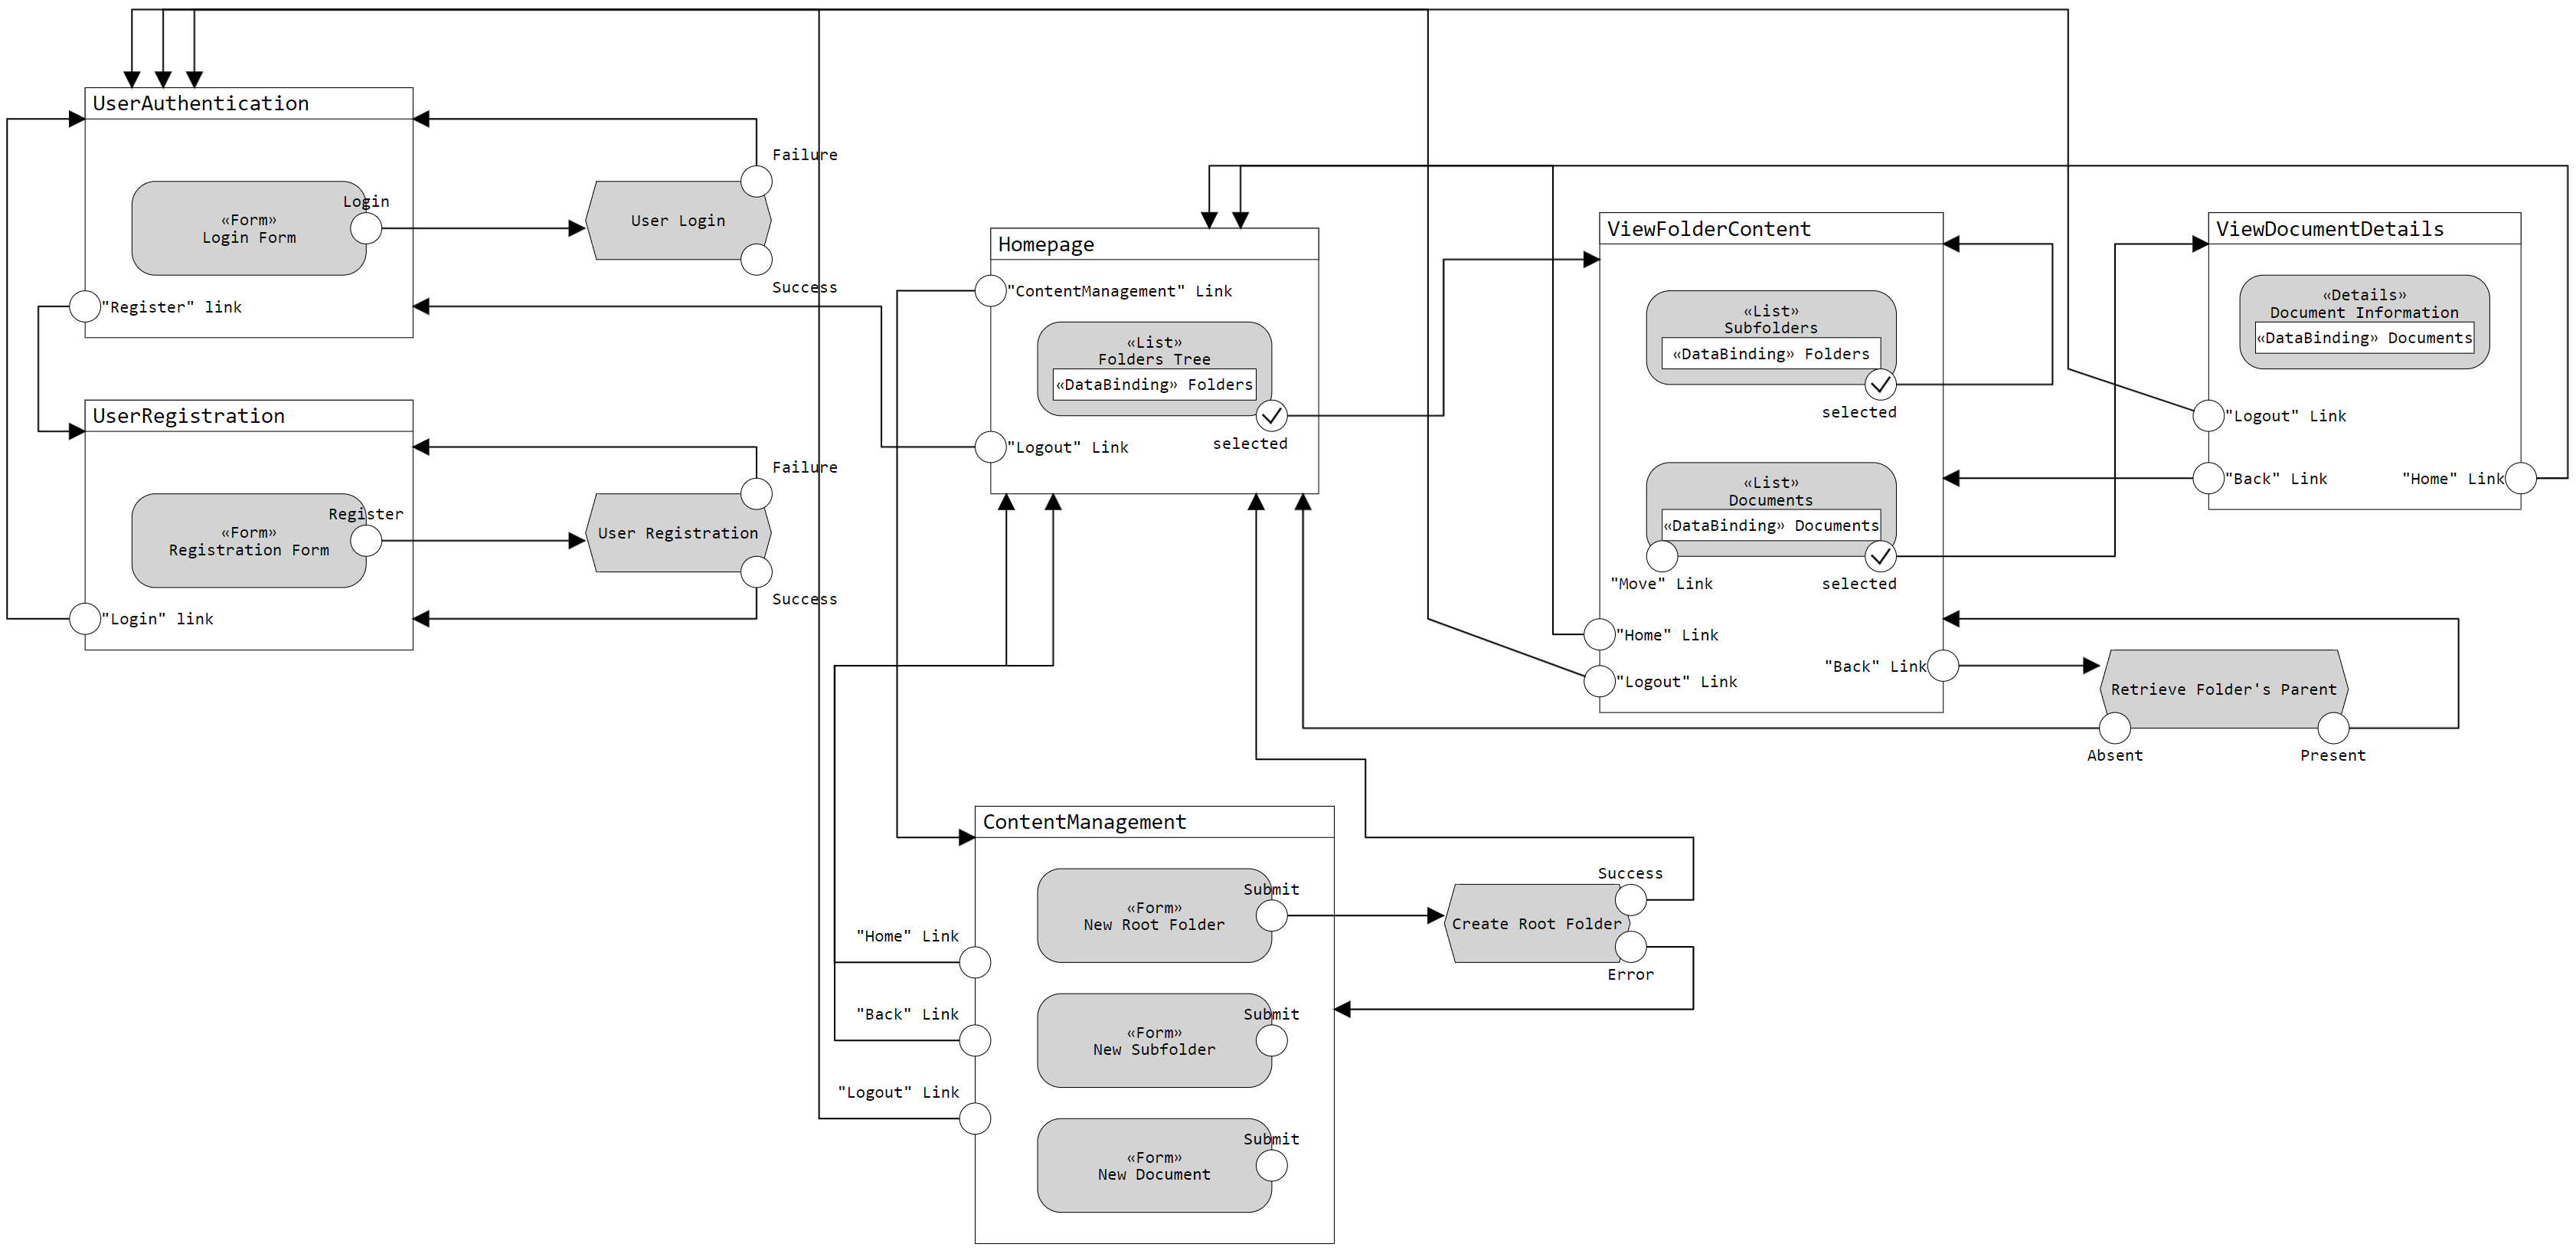
\includegraphics[width=1\linewidth]{Resources/IFMLs/images/IFML - Navigation.png}
    \end{figure}
\end{frame}

\begin{frame}
    \frametitle{Application Design - IFML Diagram (Document Move)}
    \begin{figure}
        \centering
        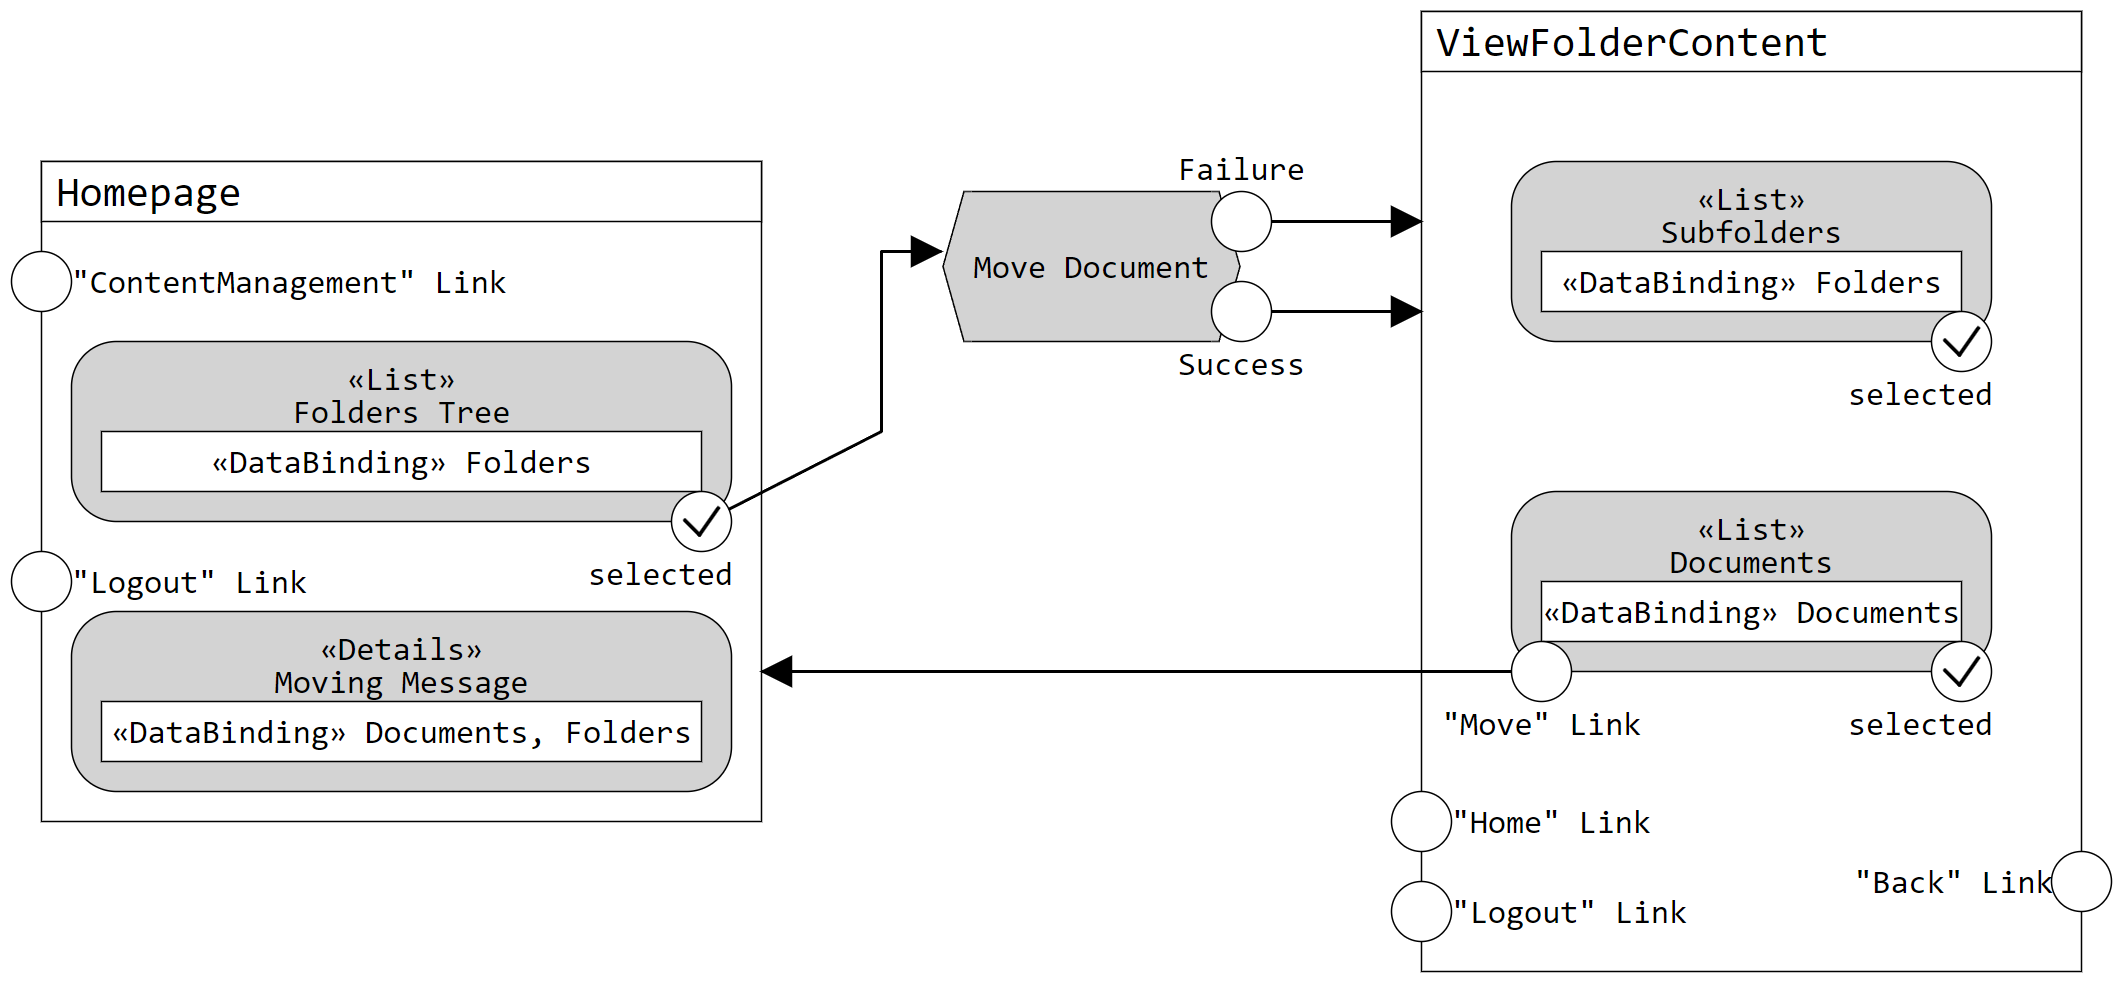
\includegraphics[width=0.9\linewidth]{Resources/IFMLs/images/IFML - Document Move.png}
    \end{figure}
\end{frame}

\begin{frame}
    \frametitle{Application Design - IFML Diagram (Subfolder Creation)}
    \begin{figure}
        \centering
        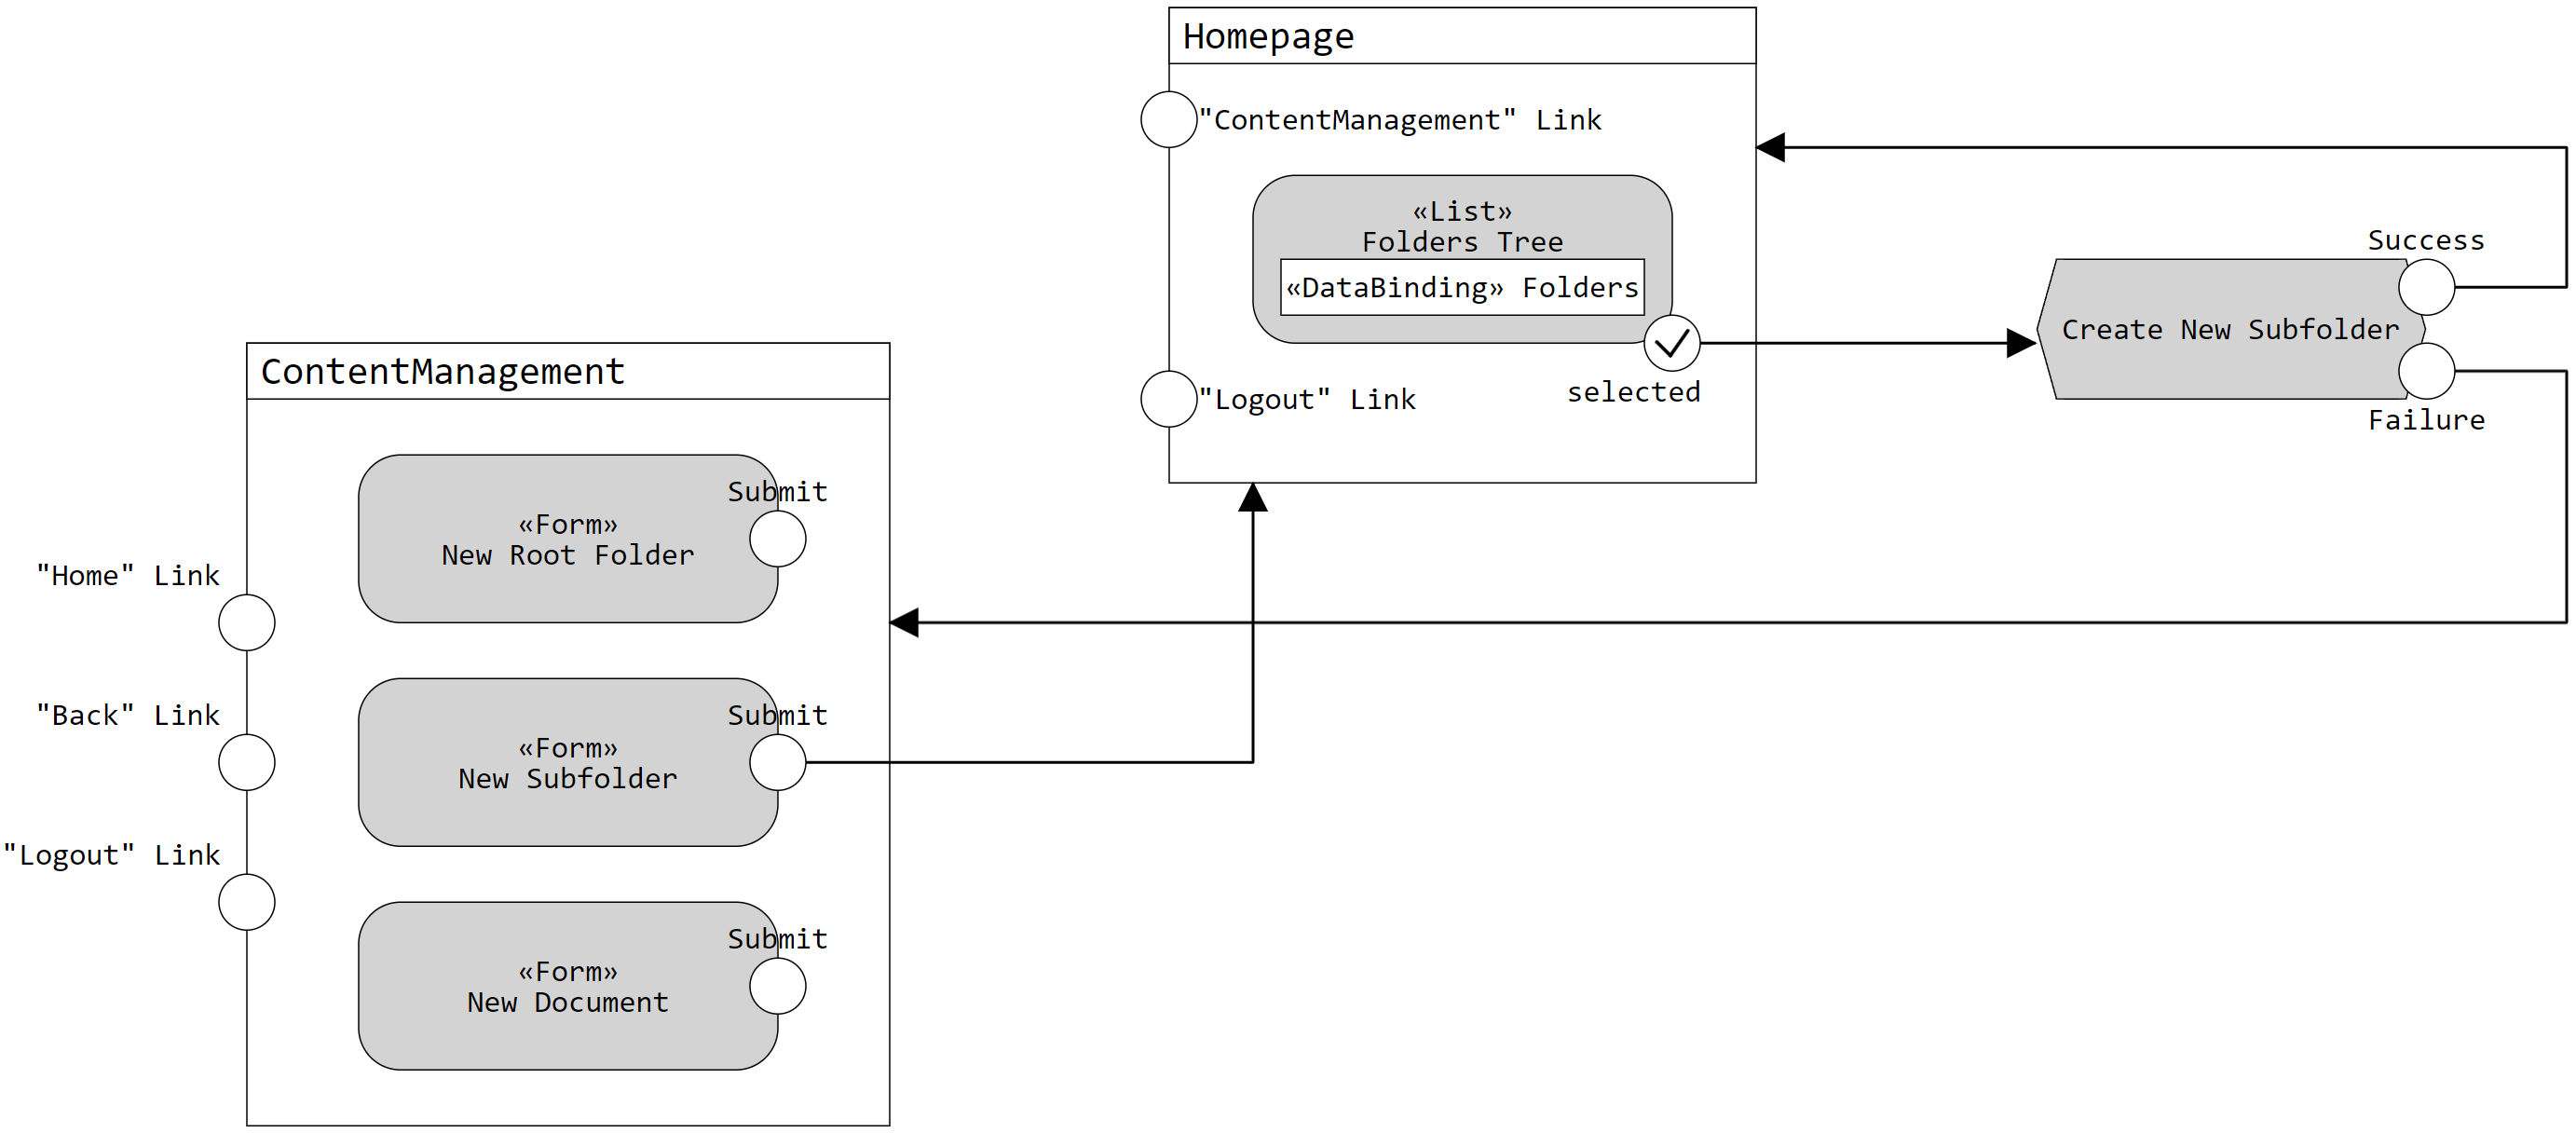
\includegraphics[width=0.9\linewidth]{Resources/IFMLs/images/IFML - Subfolder Creation.png}
    \end{figure}
\end{frame}

\begin{frame}
    \frametitle{Application Design - IFML Diagram (Document Creation)}
    \begin{figure}
        \centering
        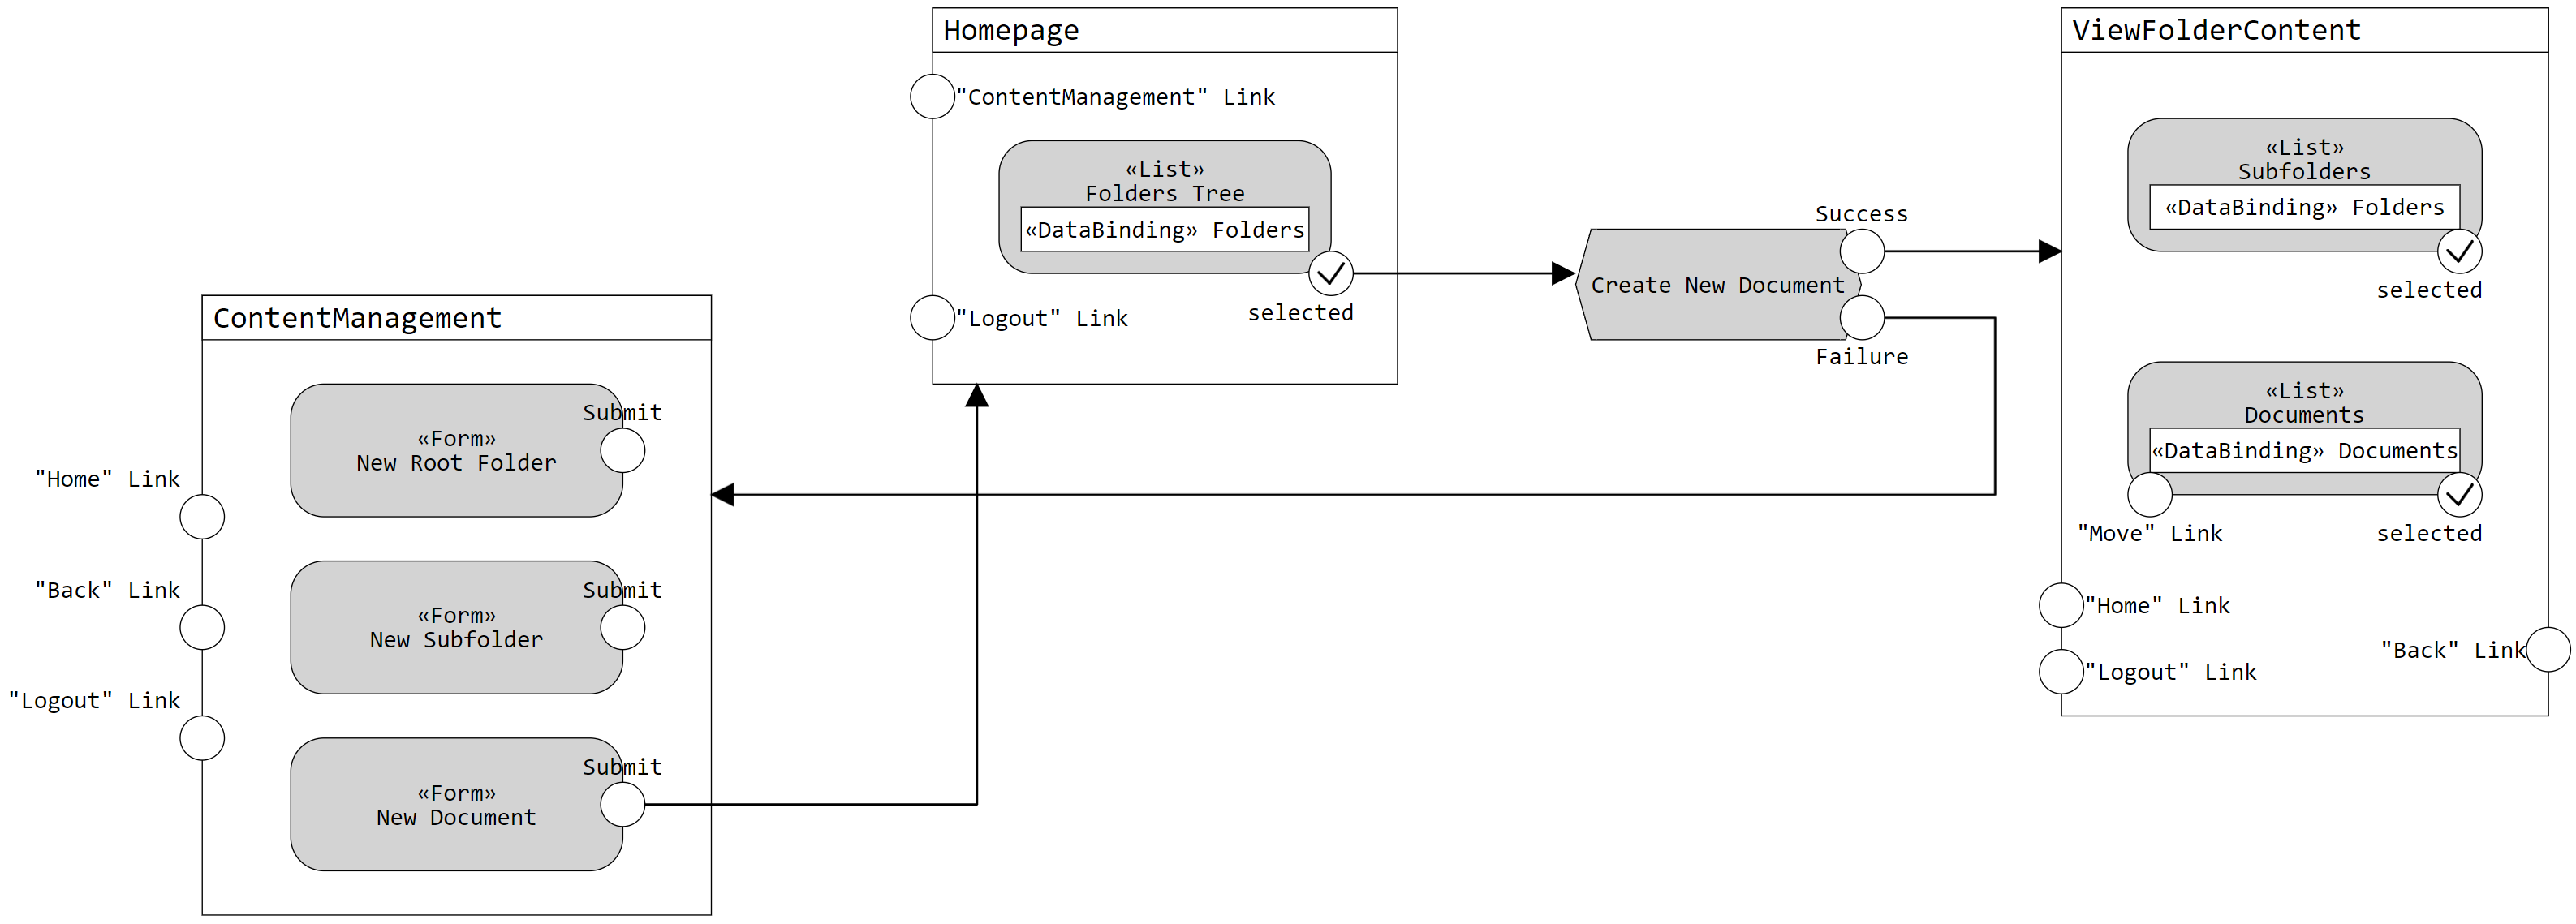
\includegraphics[width=0.9\linewidth]{Resources/IFMLs/images/IFML - Document Creation.png}
    \end{figure}
\end{frame}

\begin{frame}
    \frametitle{Application Design - Sequence Diagram}
    \begin{itemize}
        \item I diagrammi sequenziali che seguiranno rappresentano il flusso applicativo dei controller volti alla
              gestione degli eventi utente.
        \item Le servlet implementano sia i metodi "POST" e "GET", tuttavia, per mantenere la leggibilità dei diagrammi,
              quando una servlet implementa uno di questi medoti come semplice wrapper rispetto all'altro (es. "GET" che
              reindirizza a "POST" senza variazione di parametri), quest'ultimo viene omesso. Viene mostrato il metodo
              "più significativo" per la servlet in questione.
        \item La presentazione seguirà l'ordine individuato nella tabella dei componenti.
    \end{itemize}
\end{frame}

\begin{frame}
    \begin{figure}
        \centering
        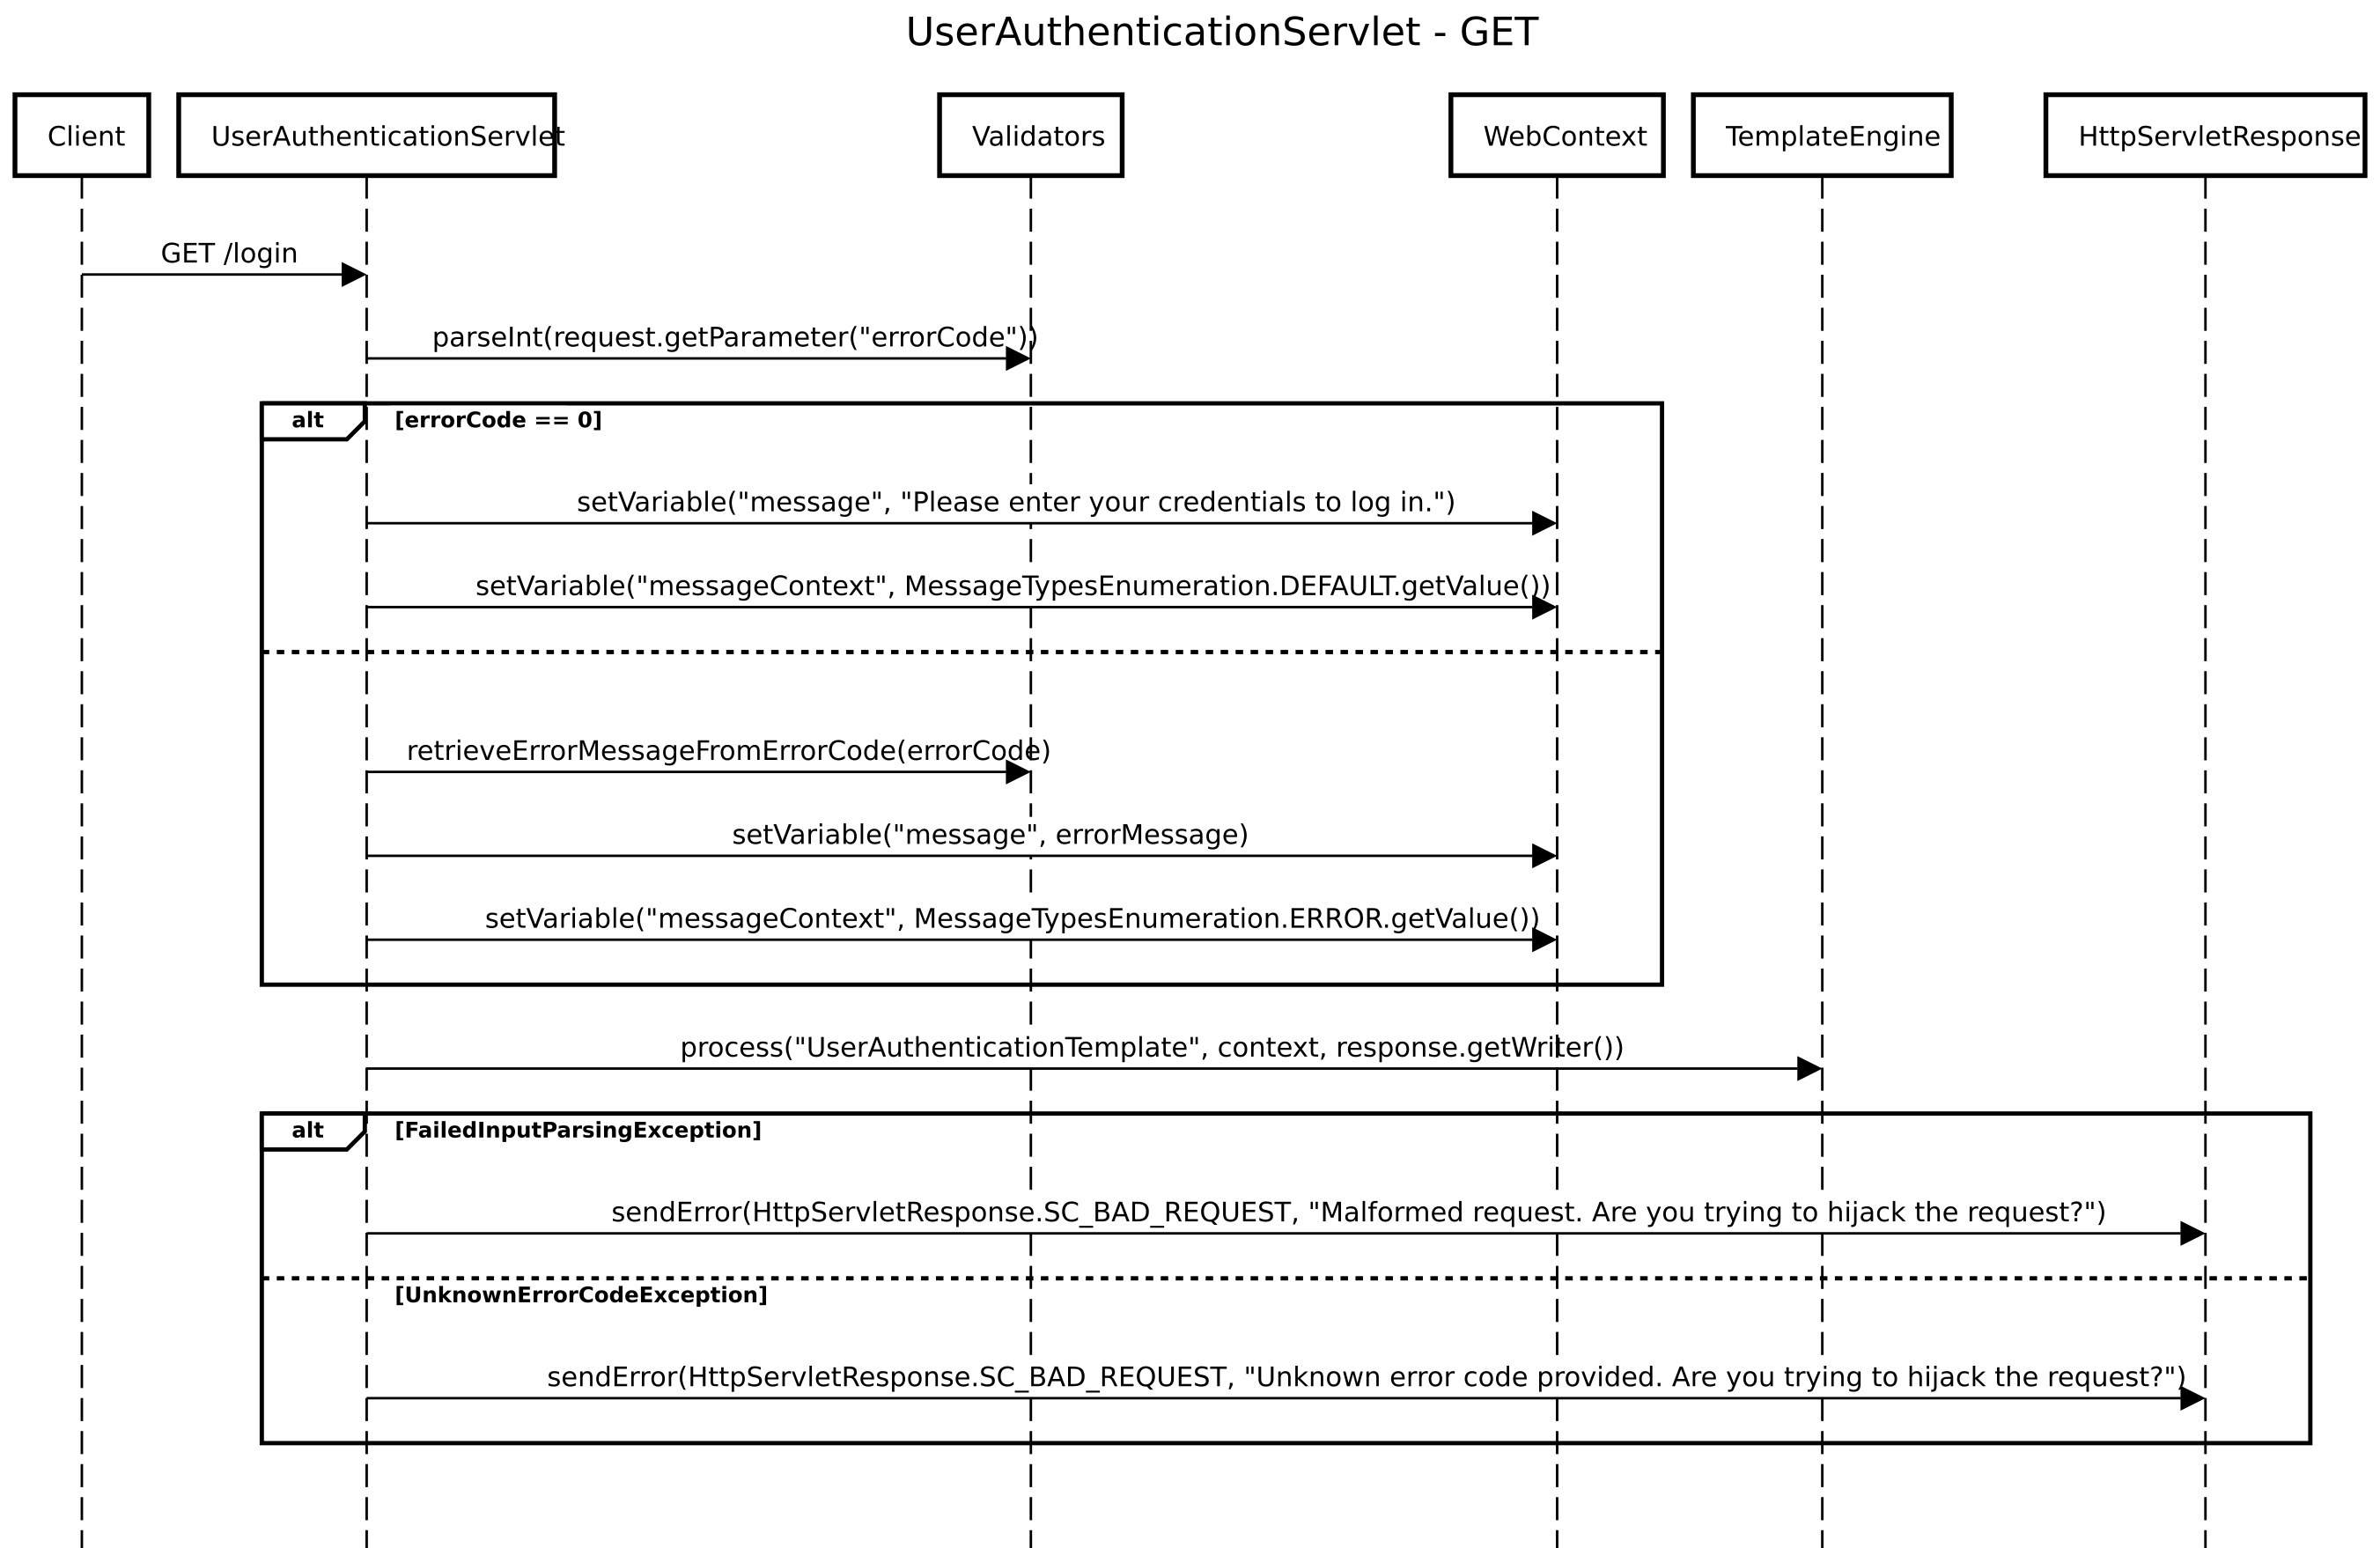
\includegraphics[width=\dimexpr 0.95\paperwidth\relax, height=\dimexpr 0.90\paperheight\relax,
            keepaspectratio]{Resources/SequenceDiagrams/images/UserAuthenticationServlet - GET.png}
    \end{figure}
\end{frame}

\begin{frame}
    \begin{figure}
        \centering
        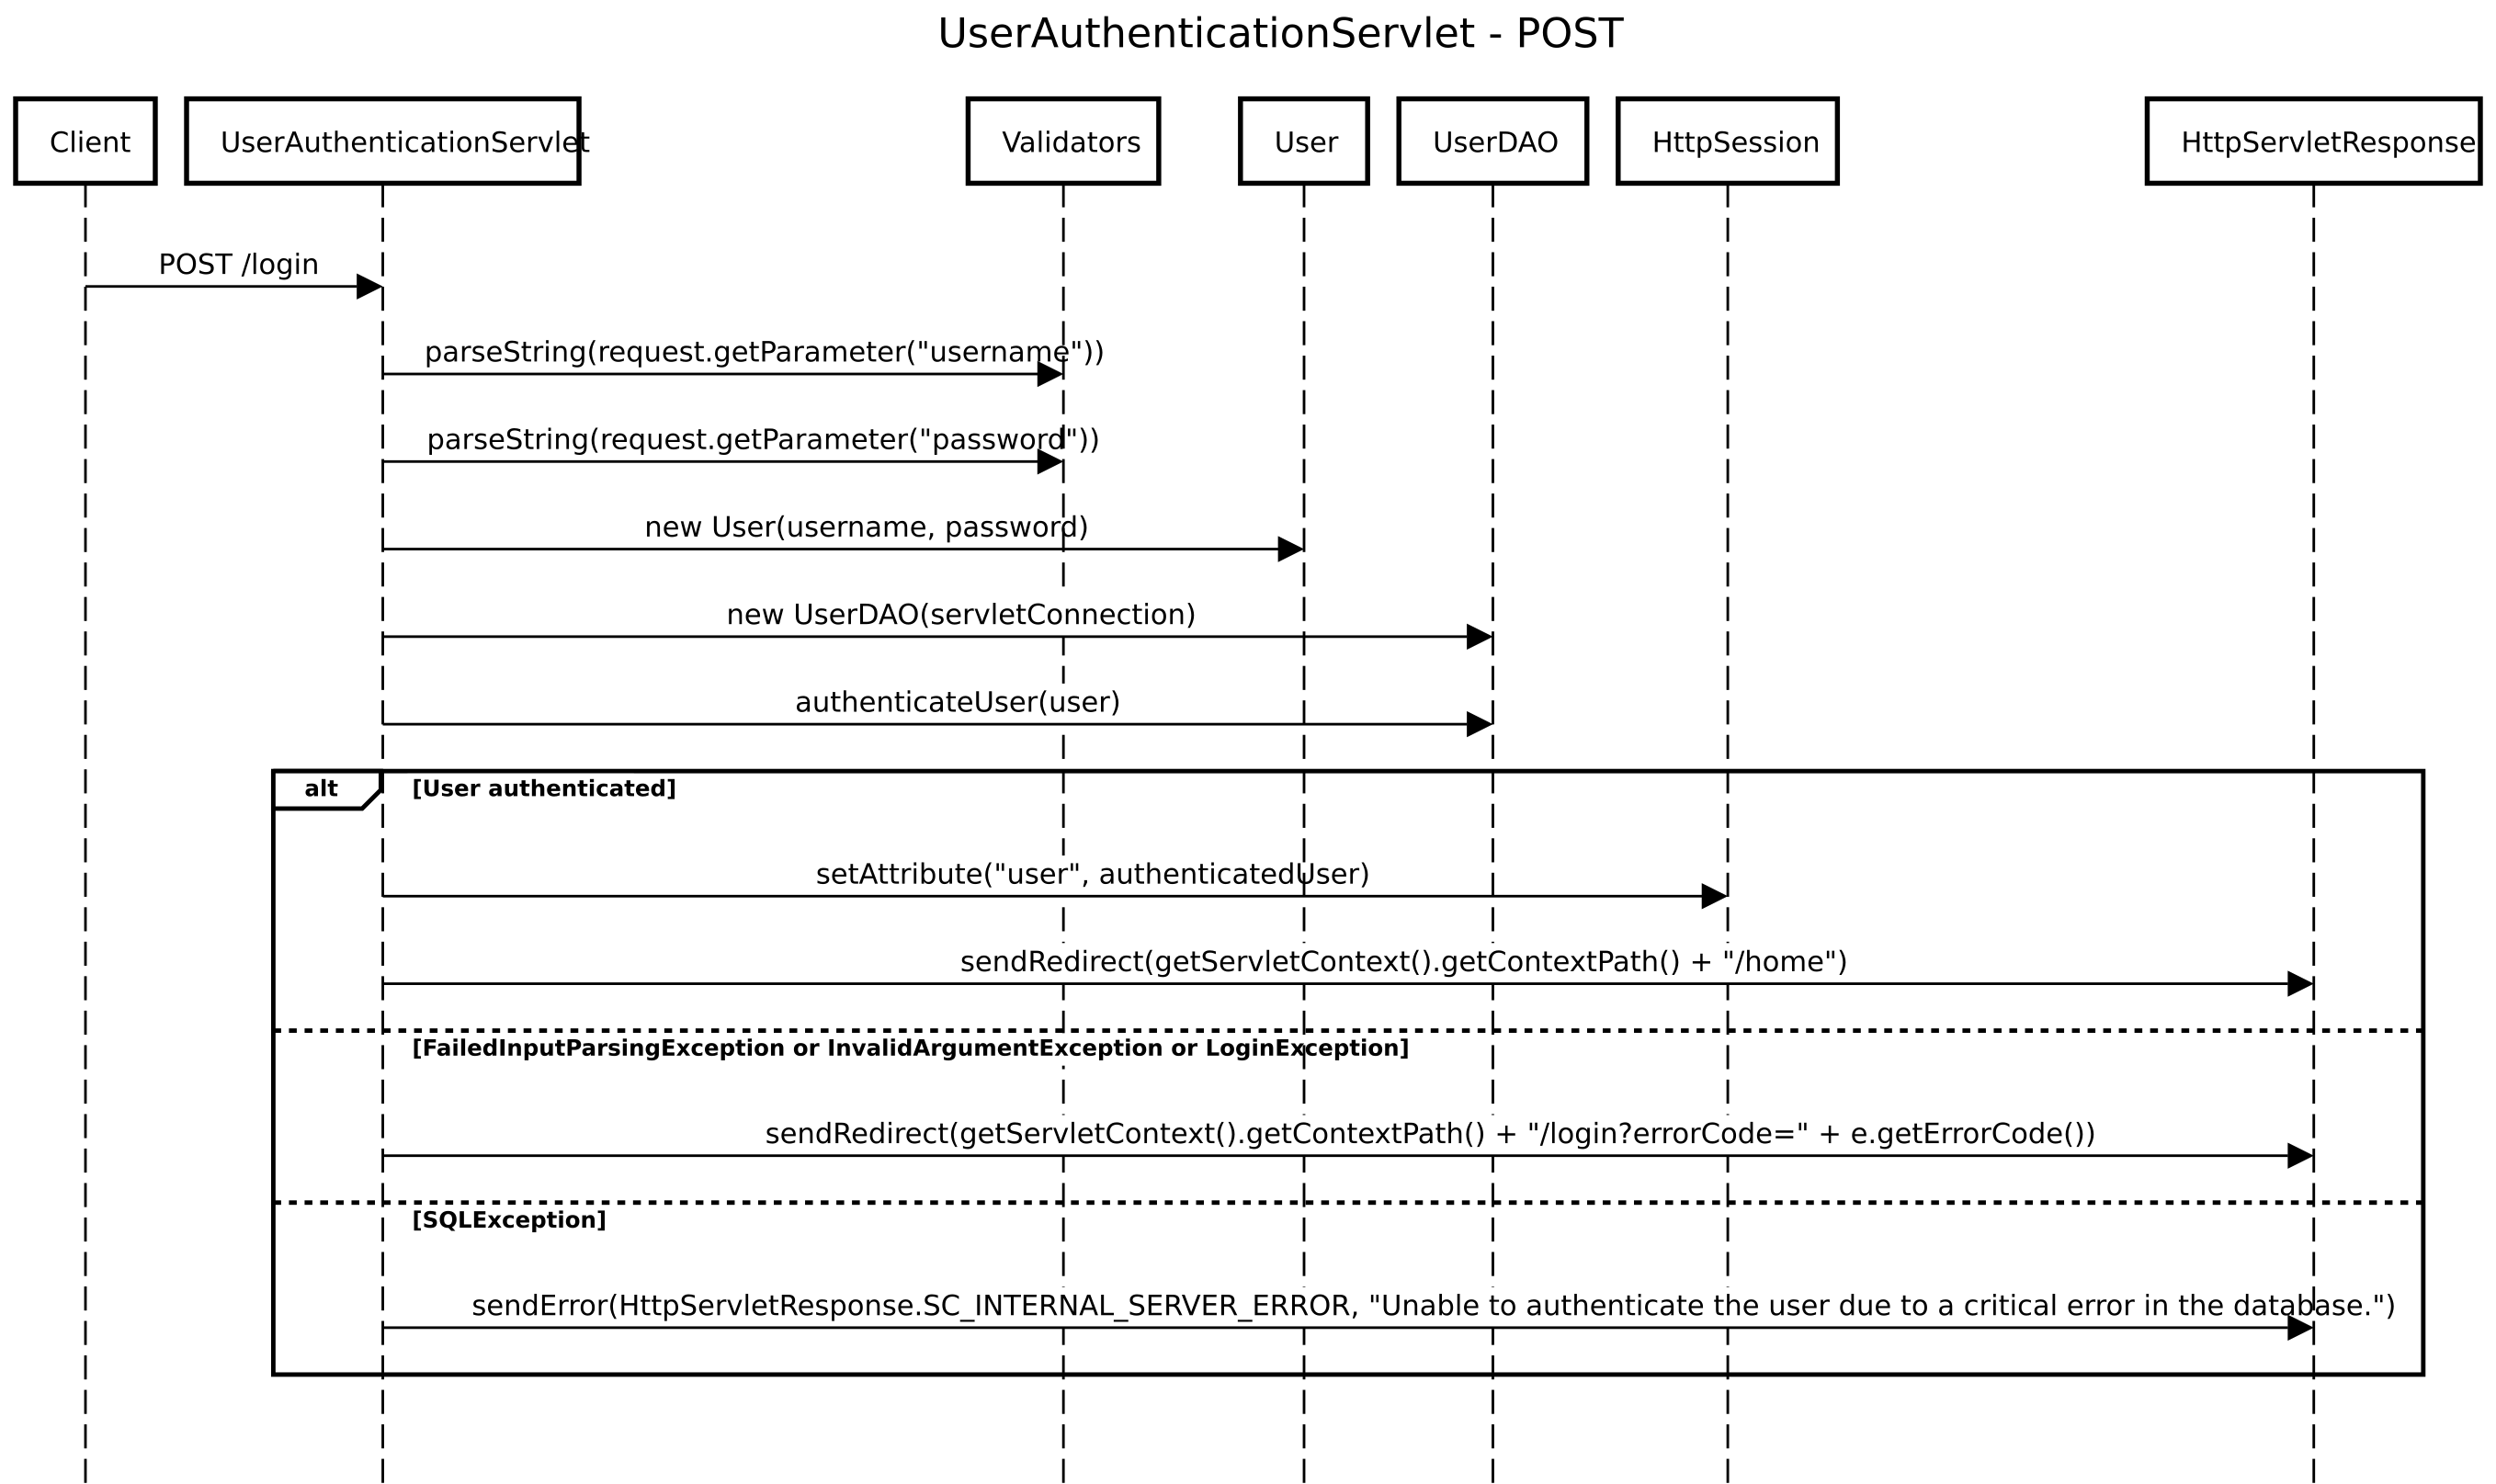
\includegraphics[width=\dimexpr 0.95\paperwidth\relax, height=\dimexpr 0.90\paperheight\relax,
            keepaspectratio]{Resources/SequenceDiagrams/images/UserAuthenticationServlet - POST.png}
    \end{figure}
\end{frame}

\begin{frame}
    \begin{figure}
        \centering
        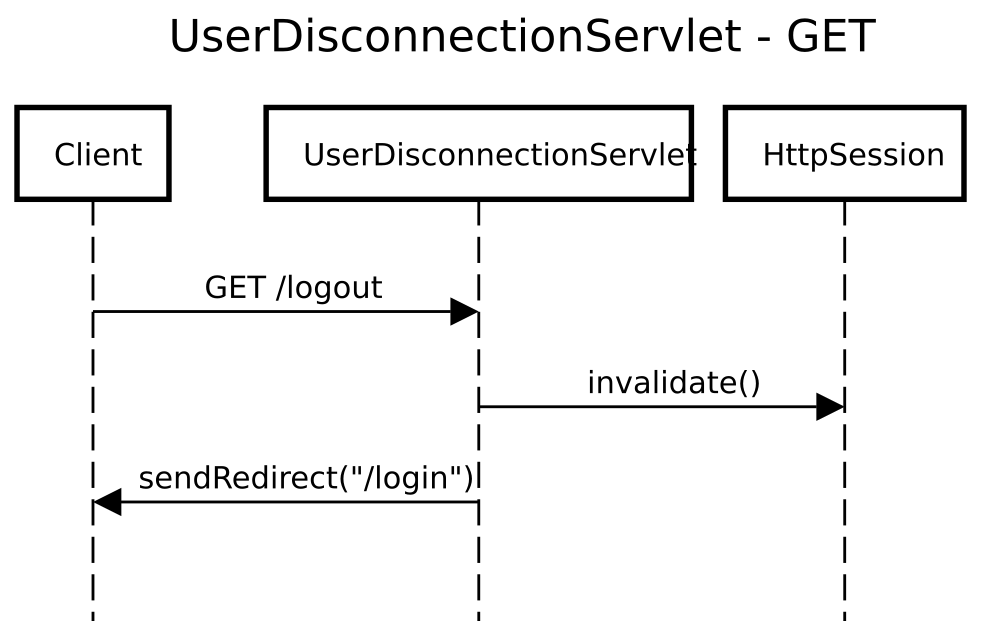
\includegraphics[width=\dimexpr 0.95\paperwidth\relax, height=\dimexpr 0.90\paperheight\relax,
            keepaspectratio]{Resources/SequenceDiagrams/images/UserDisconnectionServlet - GET.png}
    \end{figure}
\end{frame}

\begin{frame}
    \begin{figure}
        \centering
        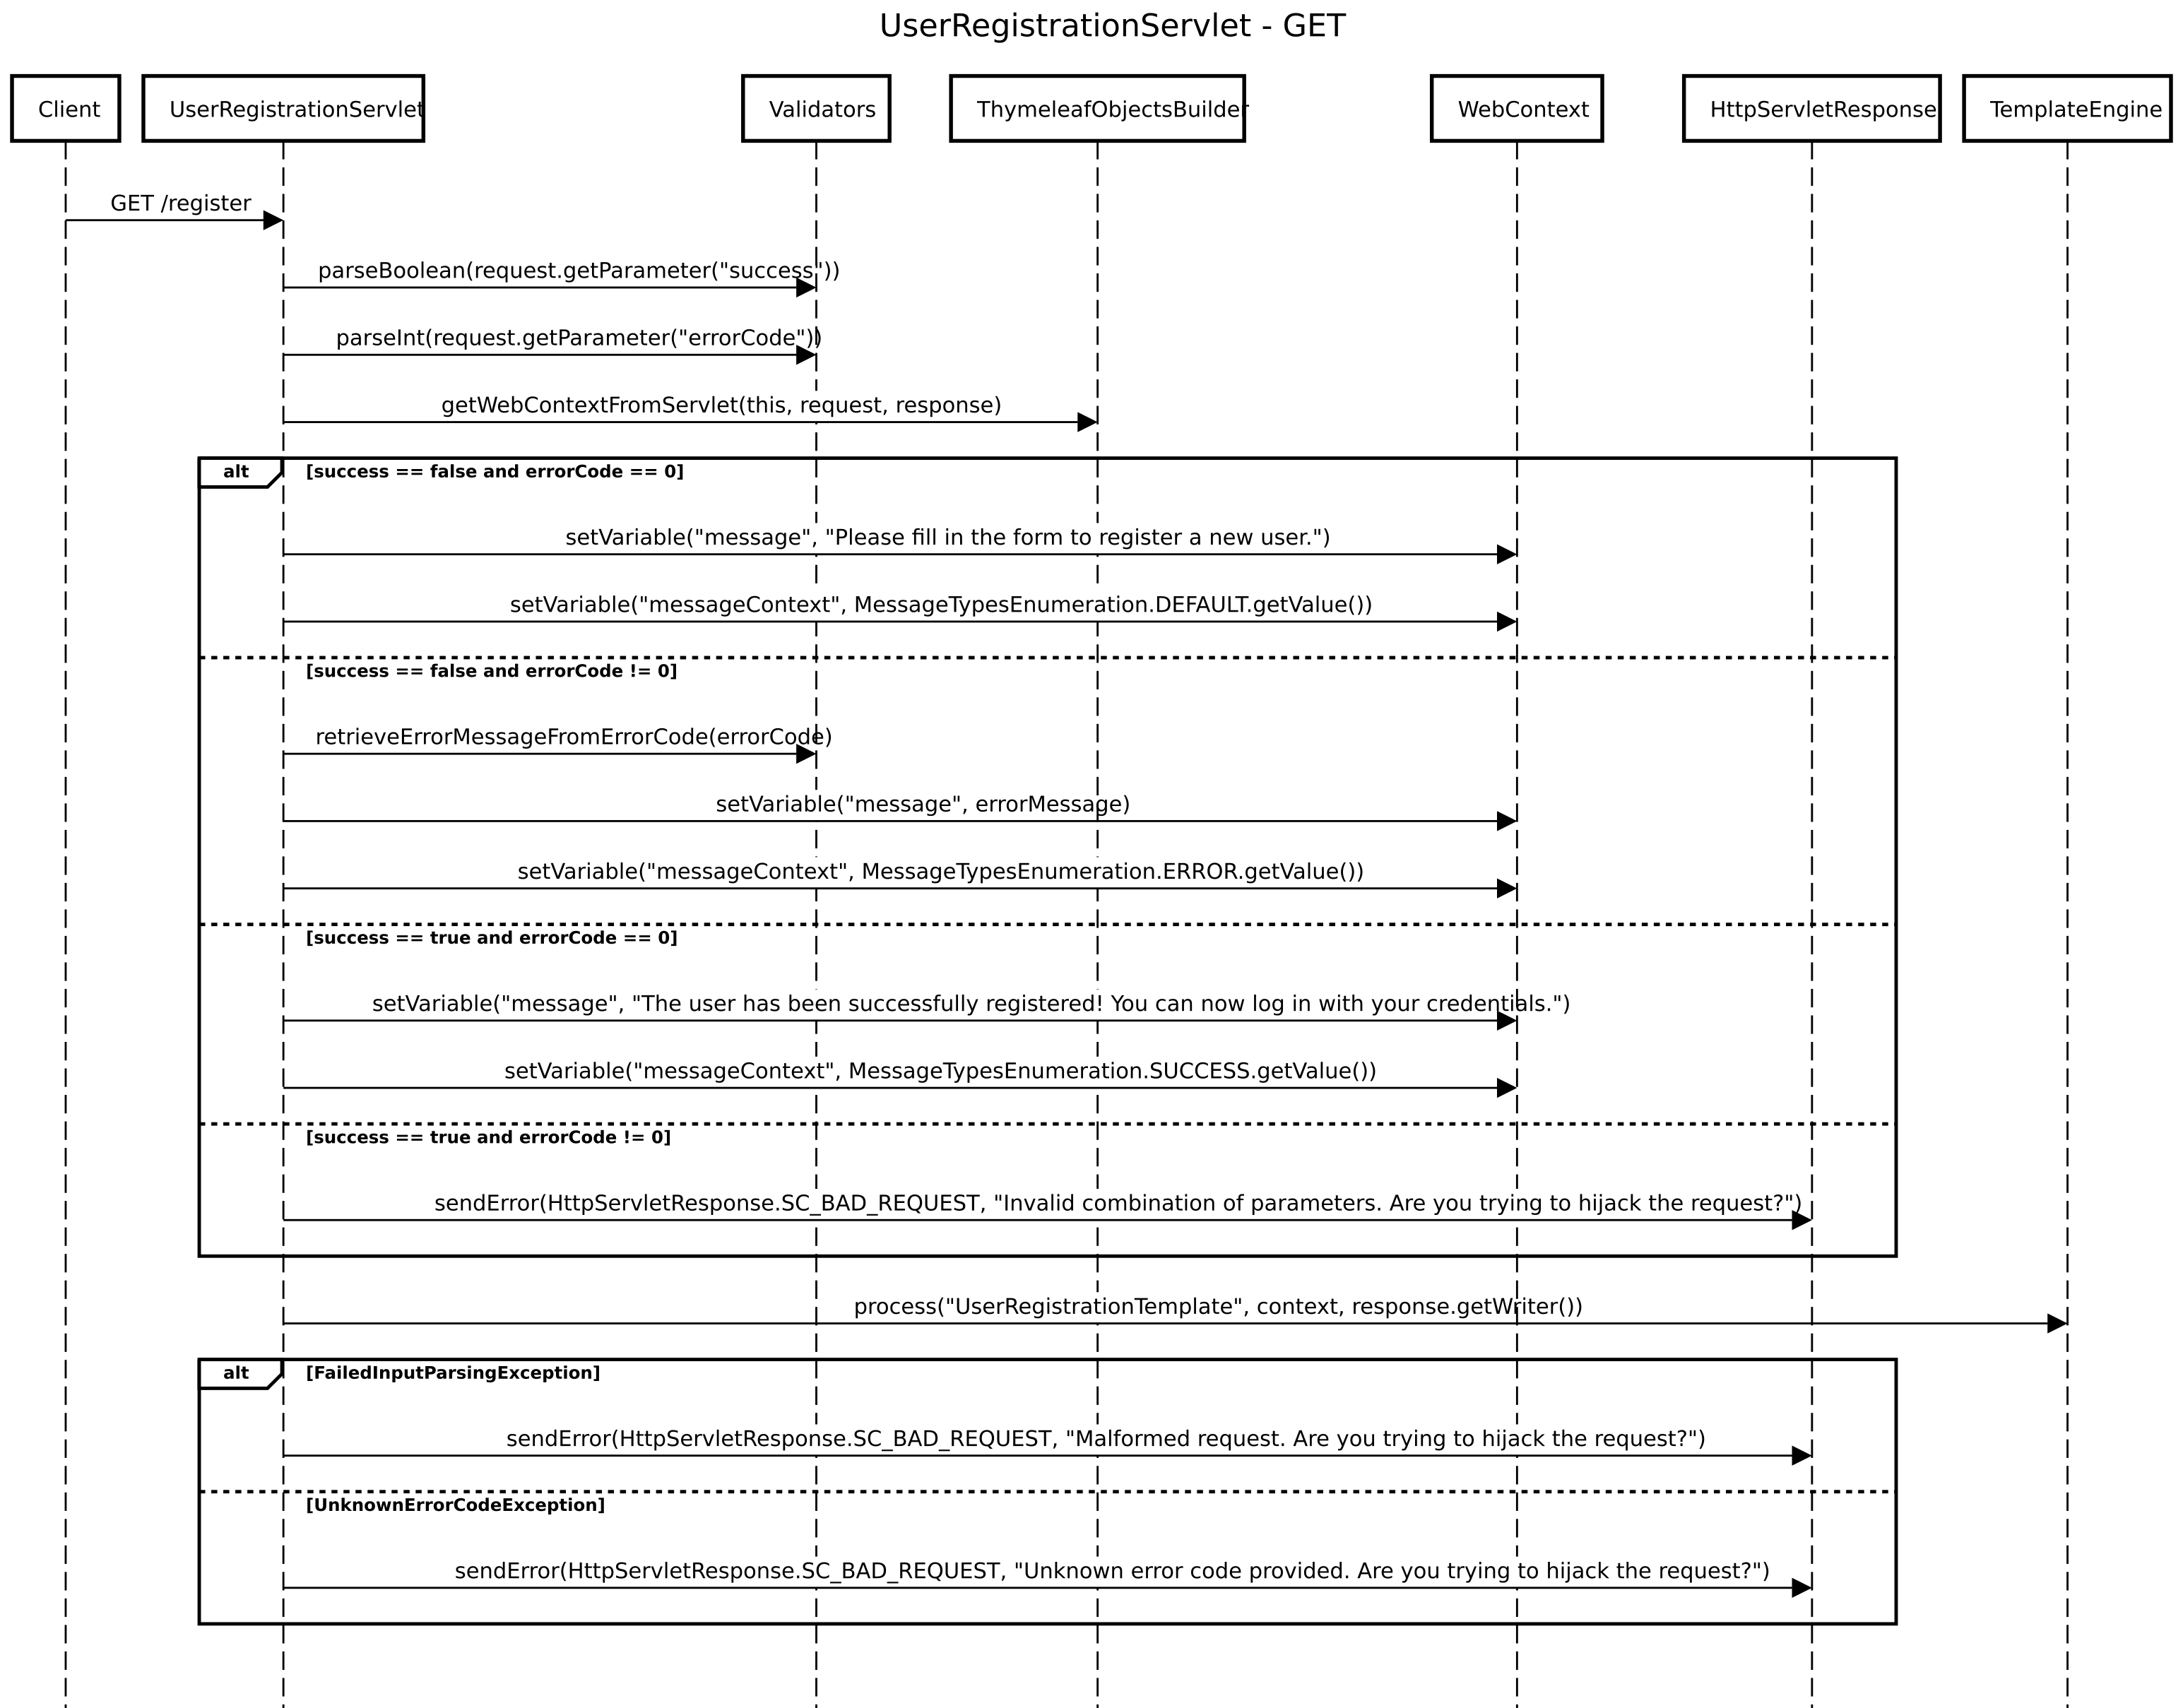
\includegraphics[width=\dimexpr 0.95\paperwidth\relax, height=\dimexpr 0.90\paperheight\relax,
            keepaspectratio]{Resources/SequenceDiagrams/images/UserRegistrationServlet - GET.png}
    \end{figure}
\end{frame}

\begin{frame}
    \begin{figure}
        \centering
        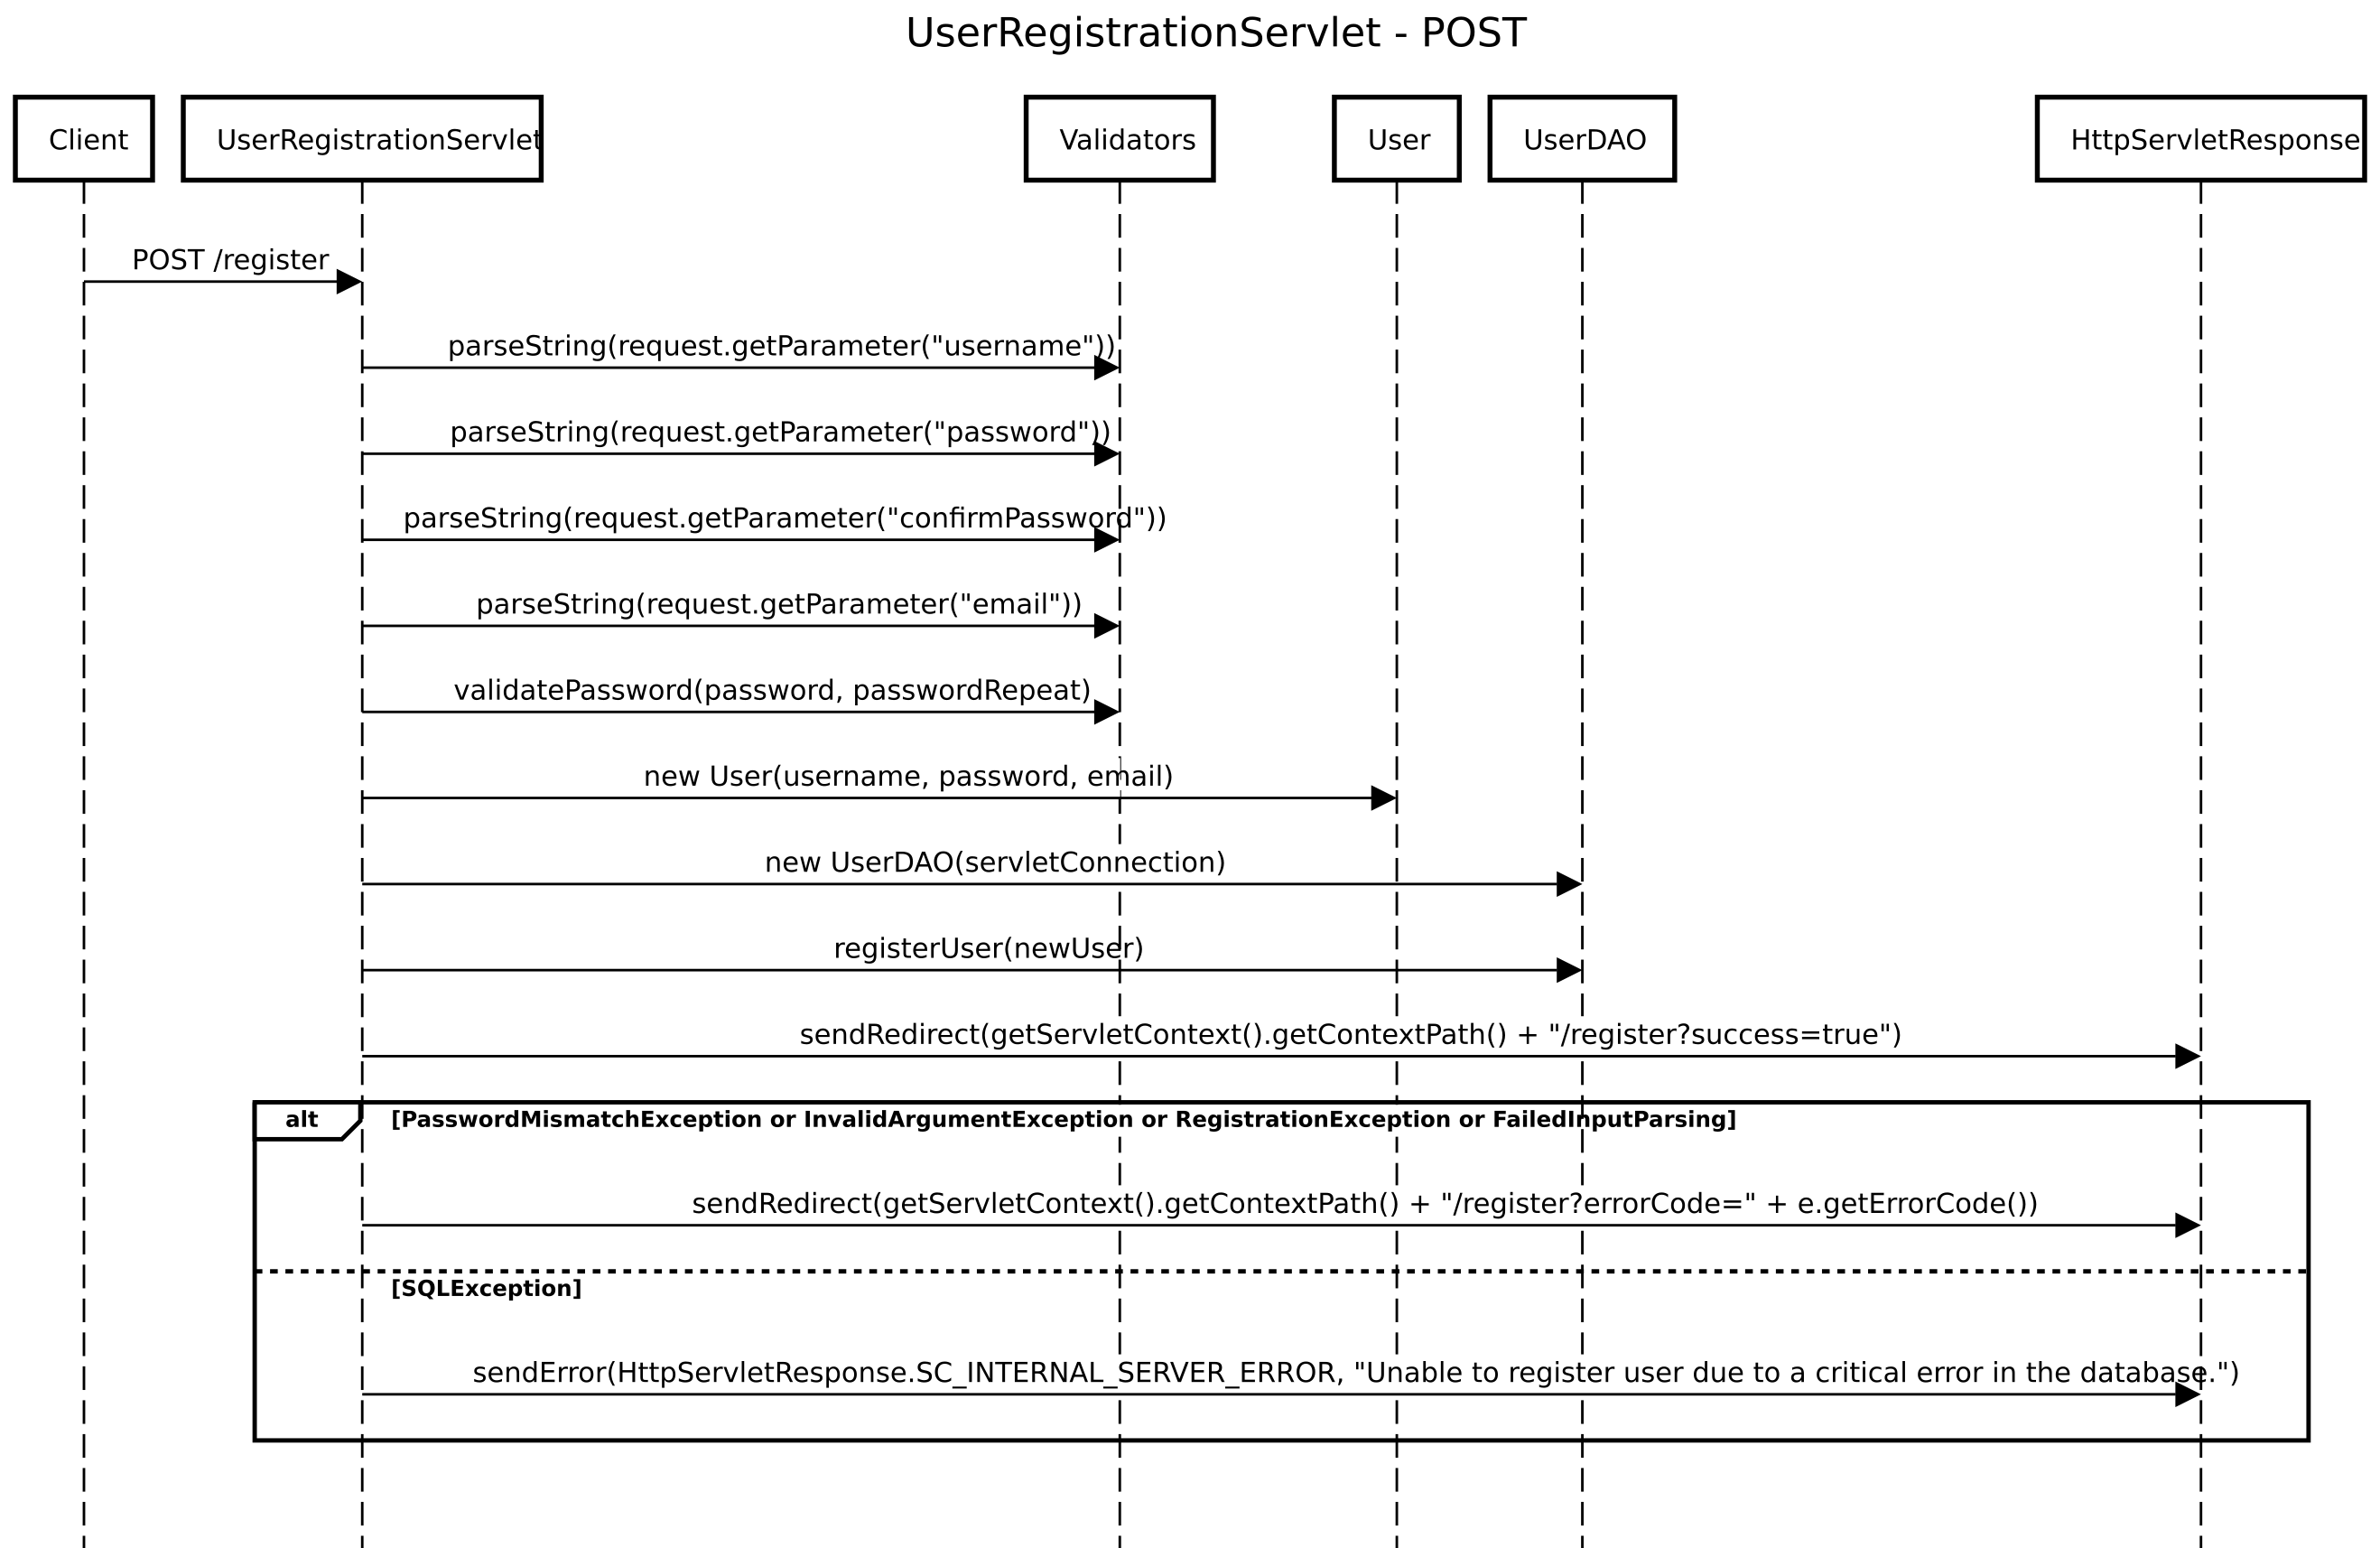
\includegraphics[width=\dimexpr 0.95\paperwidth\relax, height=\dimexpr 0.90\paperheight\relax,
            keepaspectratio]{Resources/SequenceDiagrams/images/UserRegistrationServlet - POST.png}
    \end{figure}
\end{frame}

\begin{frame}
    \begin{figure}
        \centering
        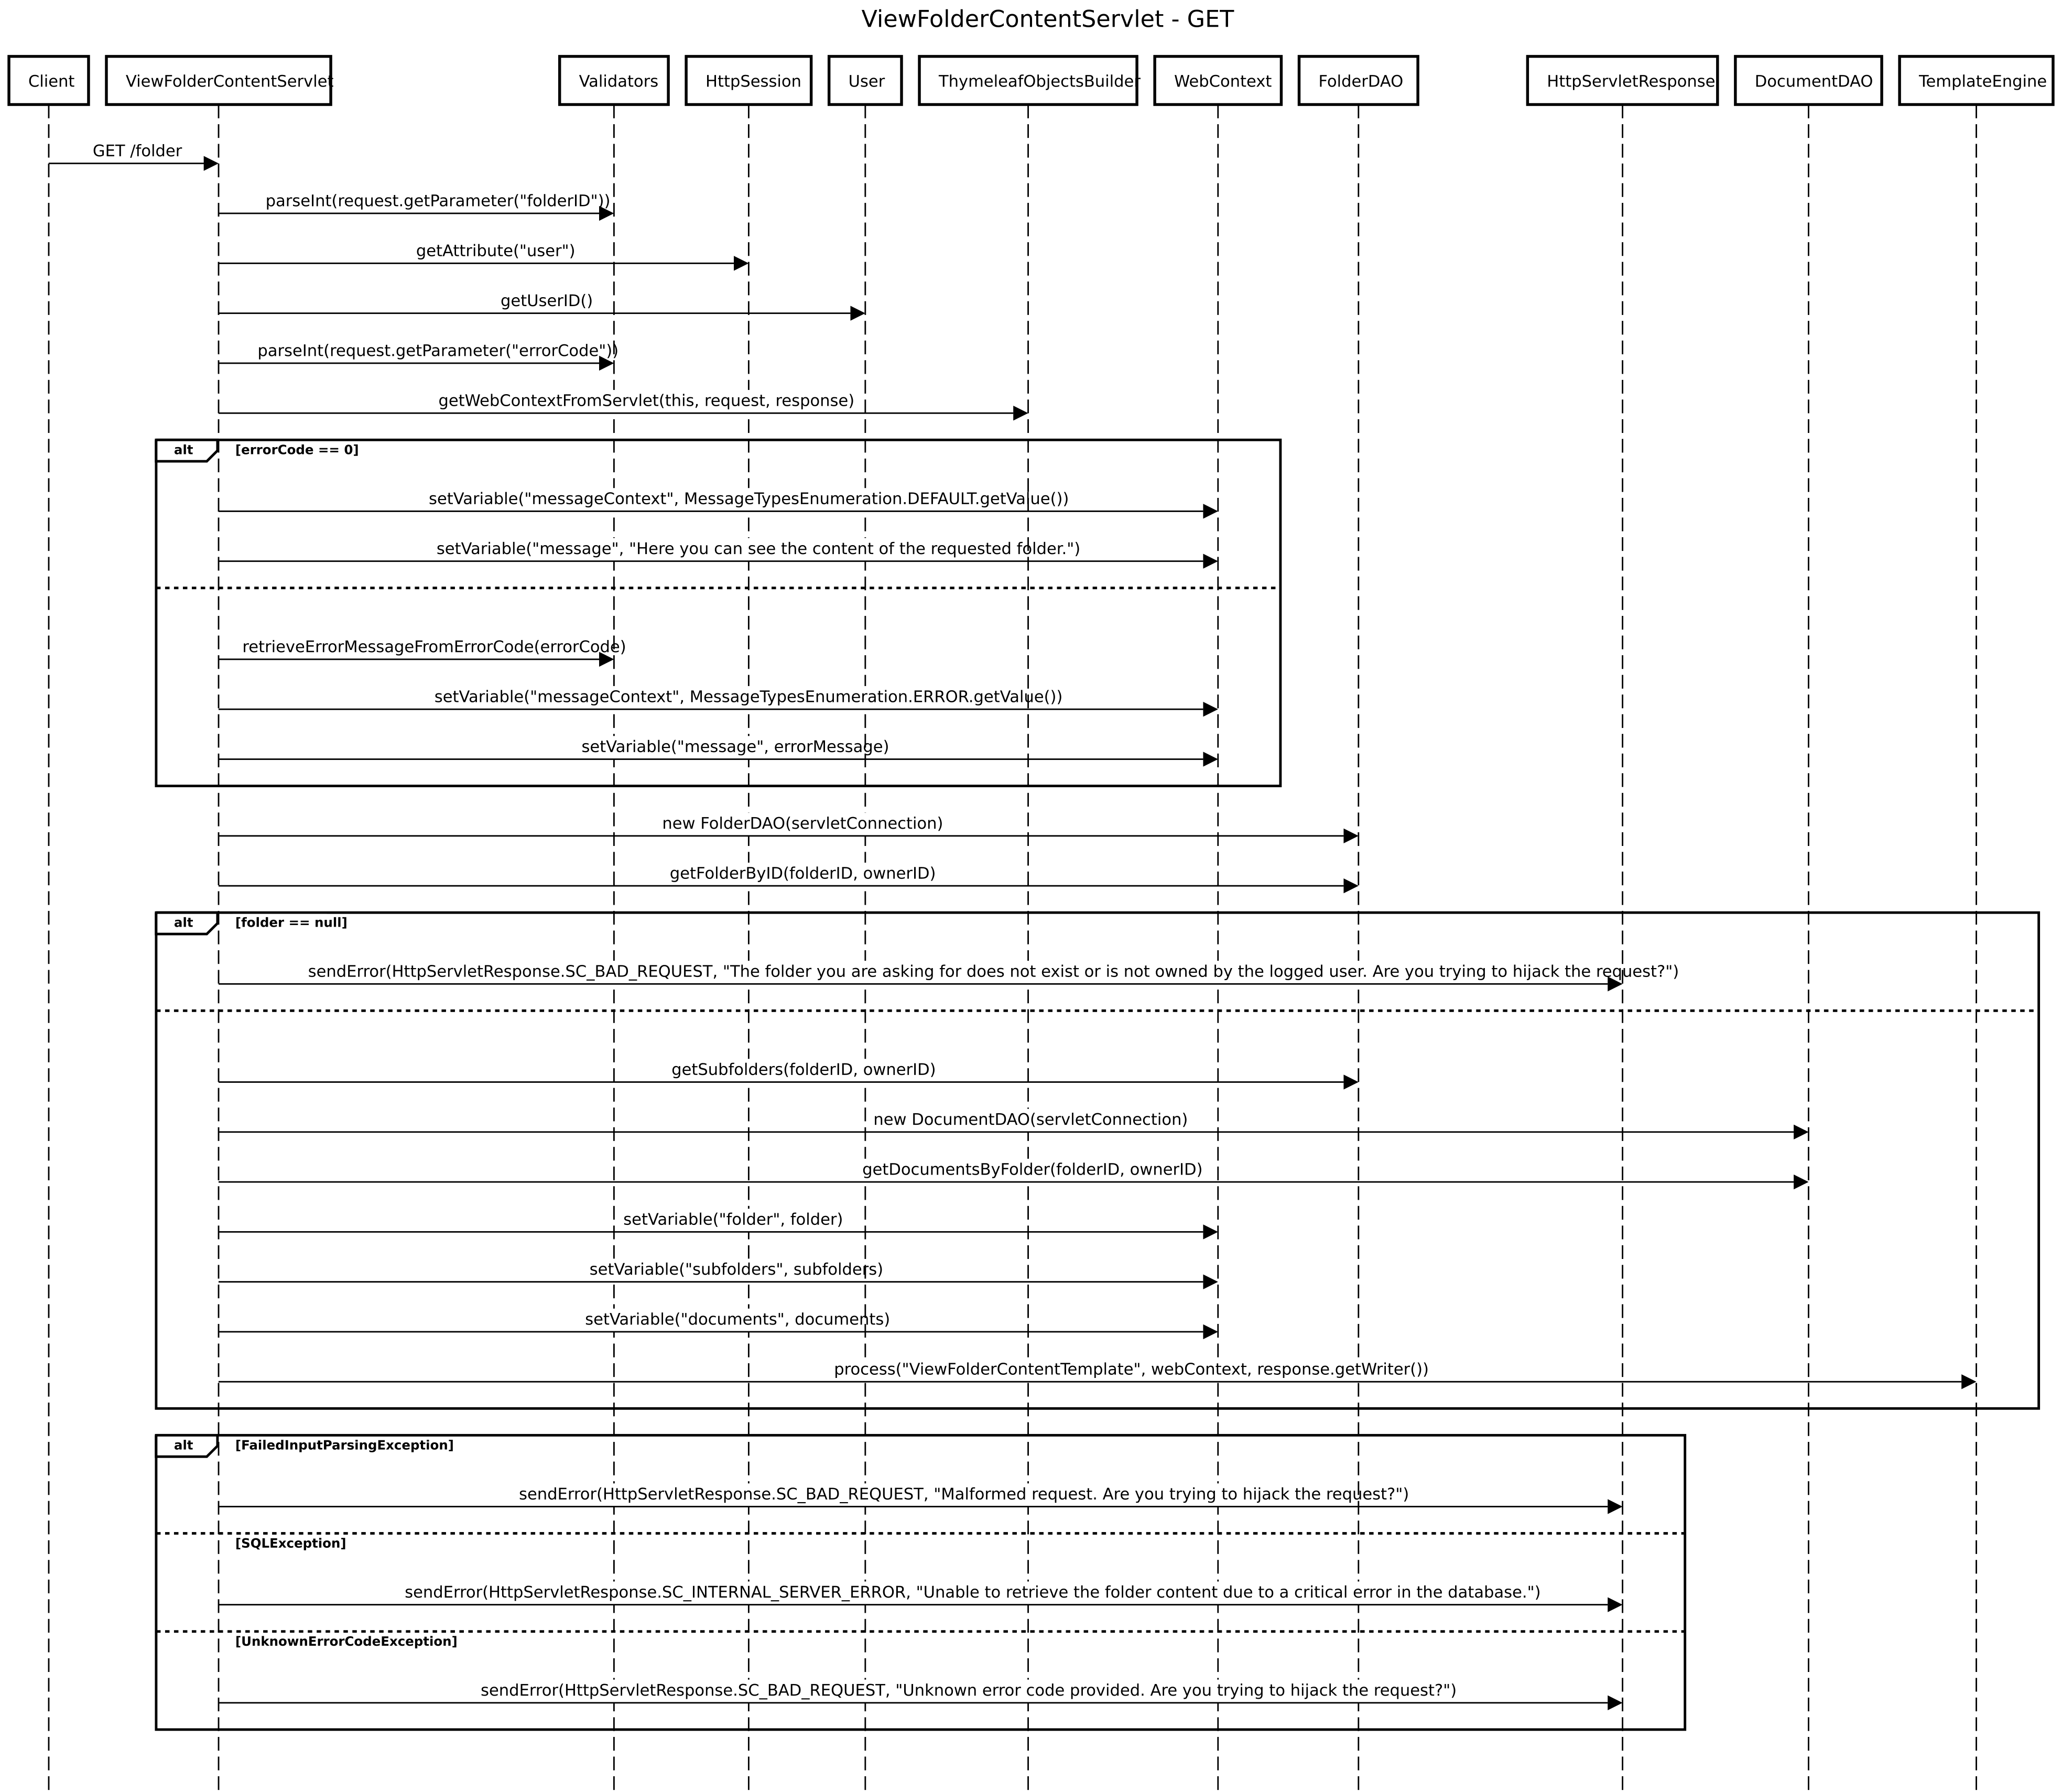
\includegraphics[width=\dimexpr 0.95\paperwidth\relax, height=\dimexpr 0.90\paperheight\relax,
            keepaspectratio]{Resources/SequenceDiagrams/images/ViewFolderContentServlet - GET.png}
    \end{figure}
\end{frame}

\begin{frame}
    \begin{figure}
        \centering
        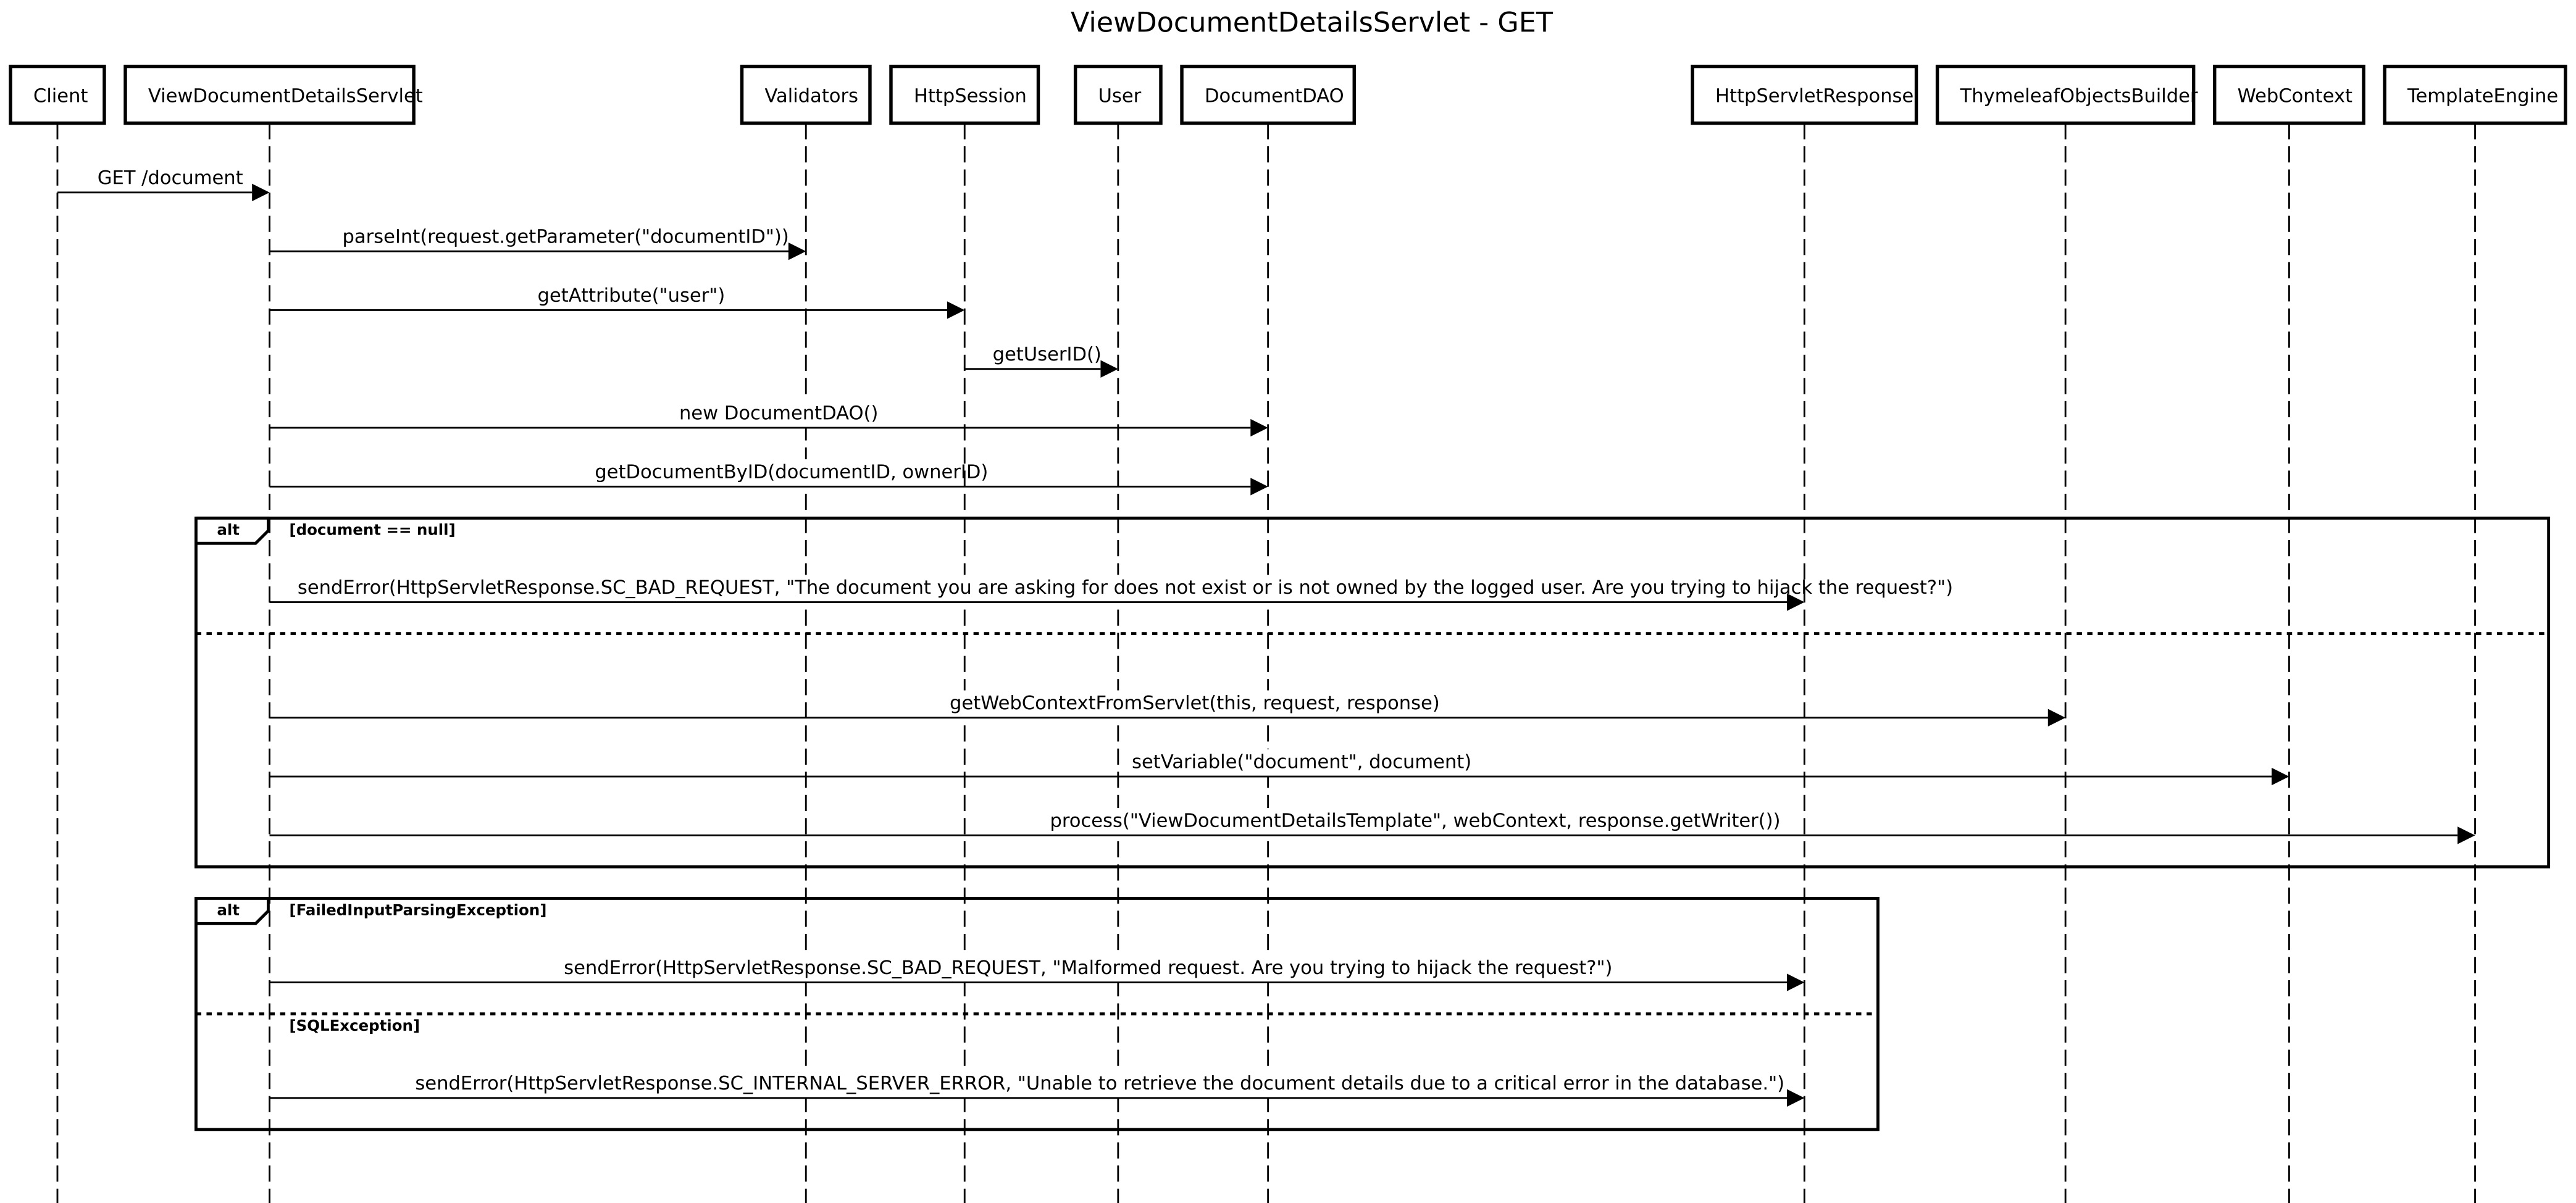
\includegraphics[width=\dimexpr 0.95\paperwidth\relax, height=\dimexpr 0.90\paperheight\relax,
            keepaspectratio]{Resources/SequenceDiagrams/images/ViewDocumentDetailsServlet - GET.png}
    \end{figure}
\end{frame}

\begin{frame}
    \begin{figure}
        \centering
        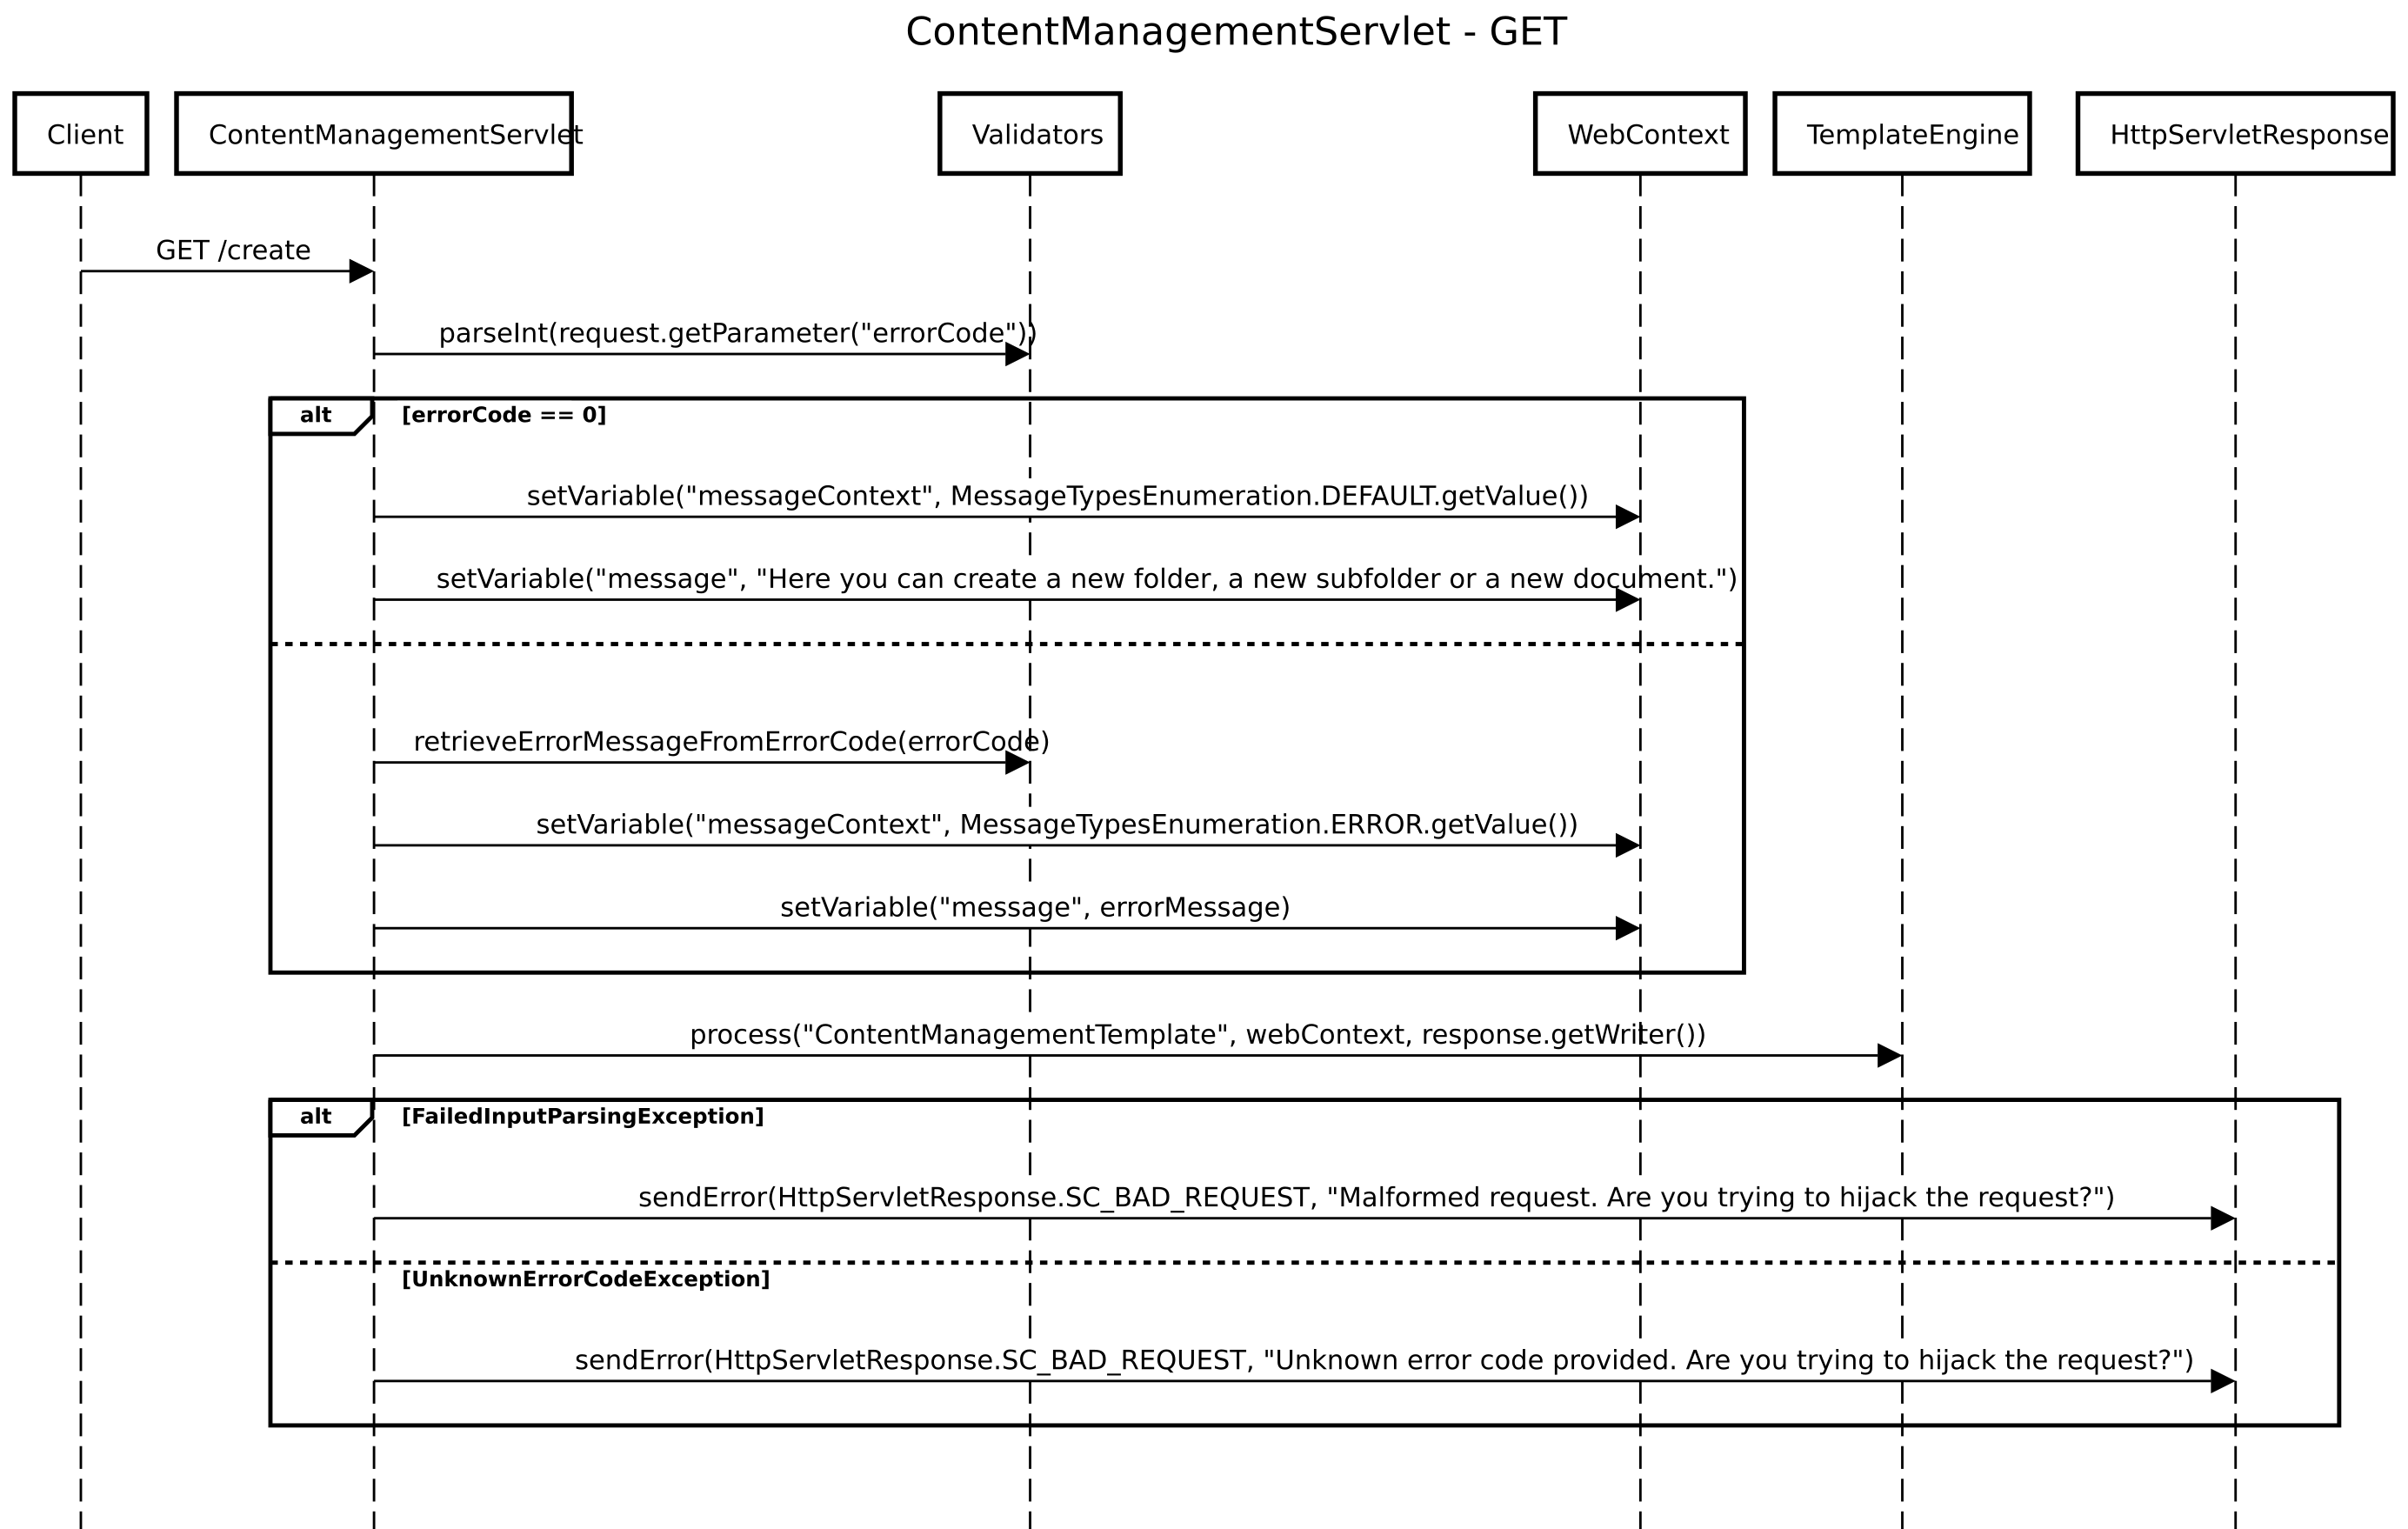
\includegraphics[width=\dimexpr 0.95\paperwidth\relax, height=\dimexpr 0.90\paperheight\relax,
            keepaspectratio]{Resources/SequenceDiagrams/images/ContentManagementServlet - GET.png}
    \end{figure}
\end{frame}

\begin{frame}
    \begin{figure}
        \centering
        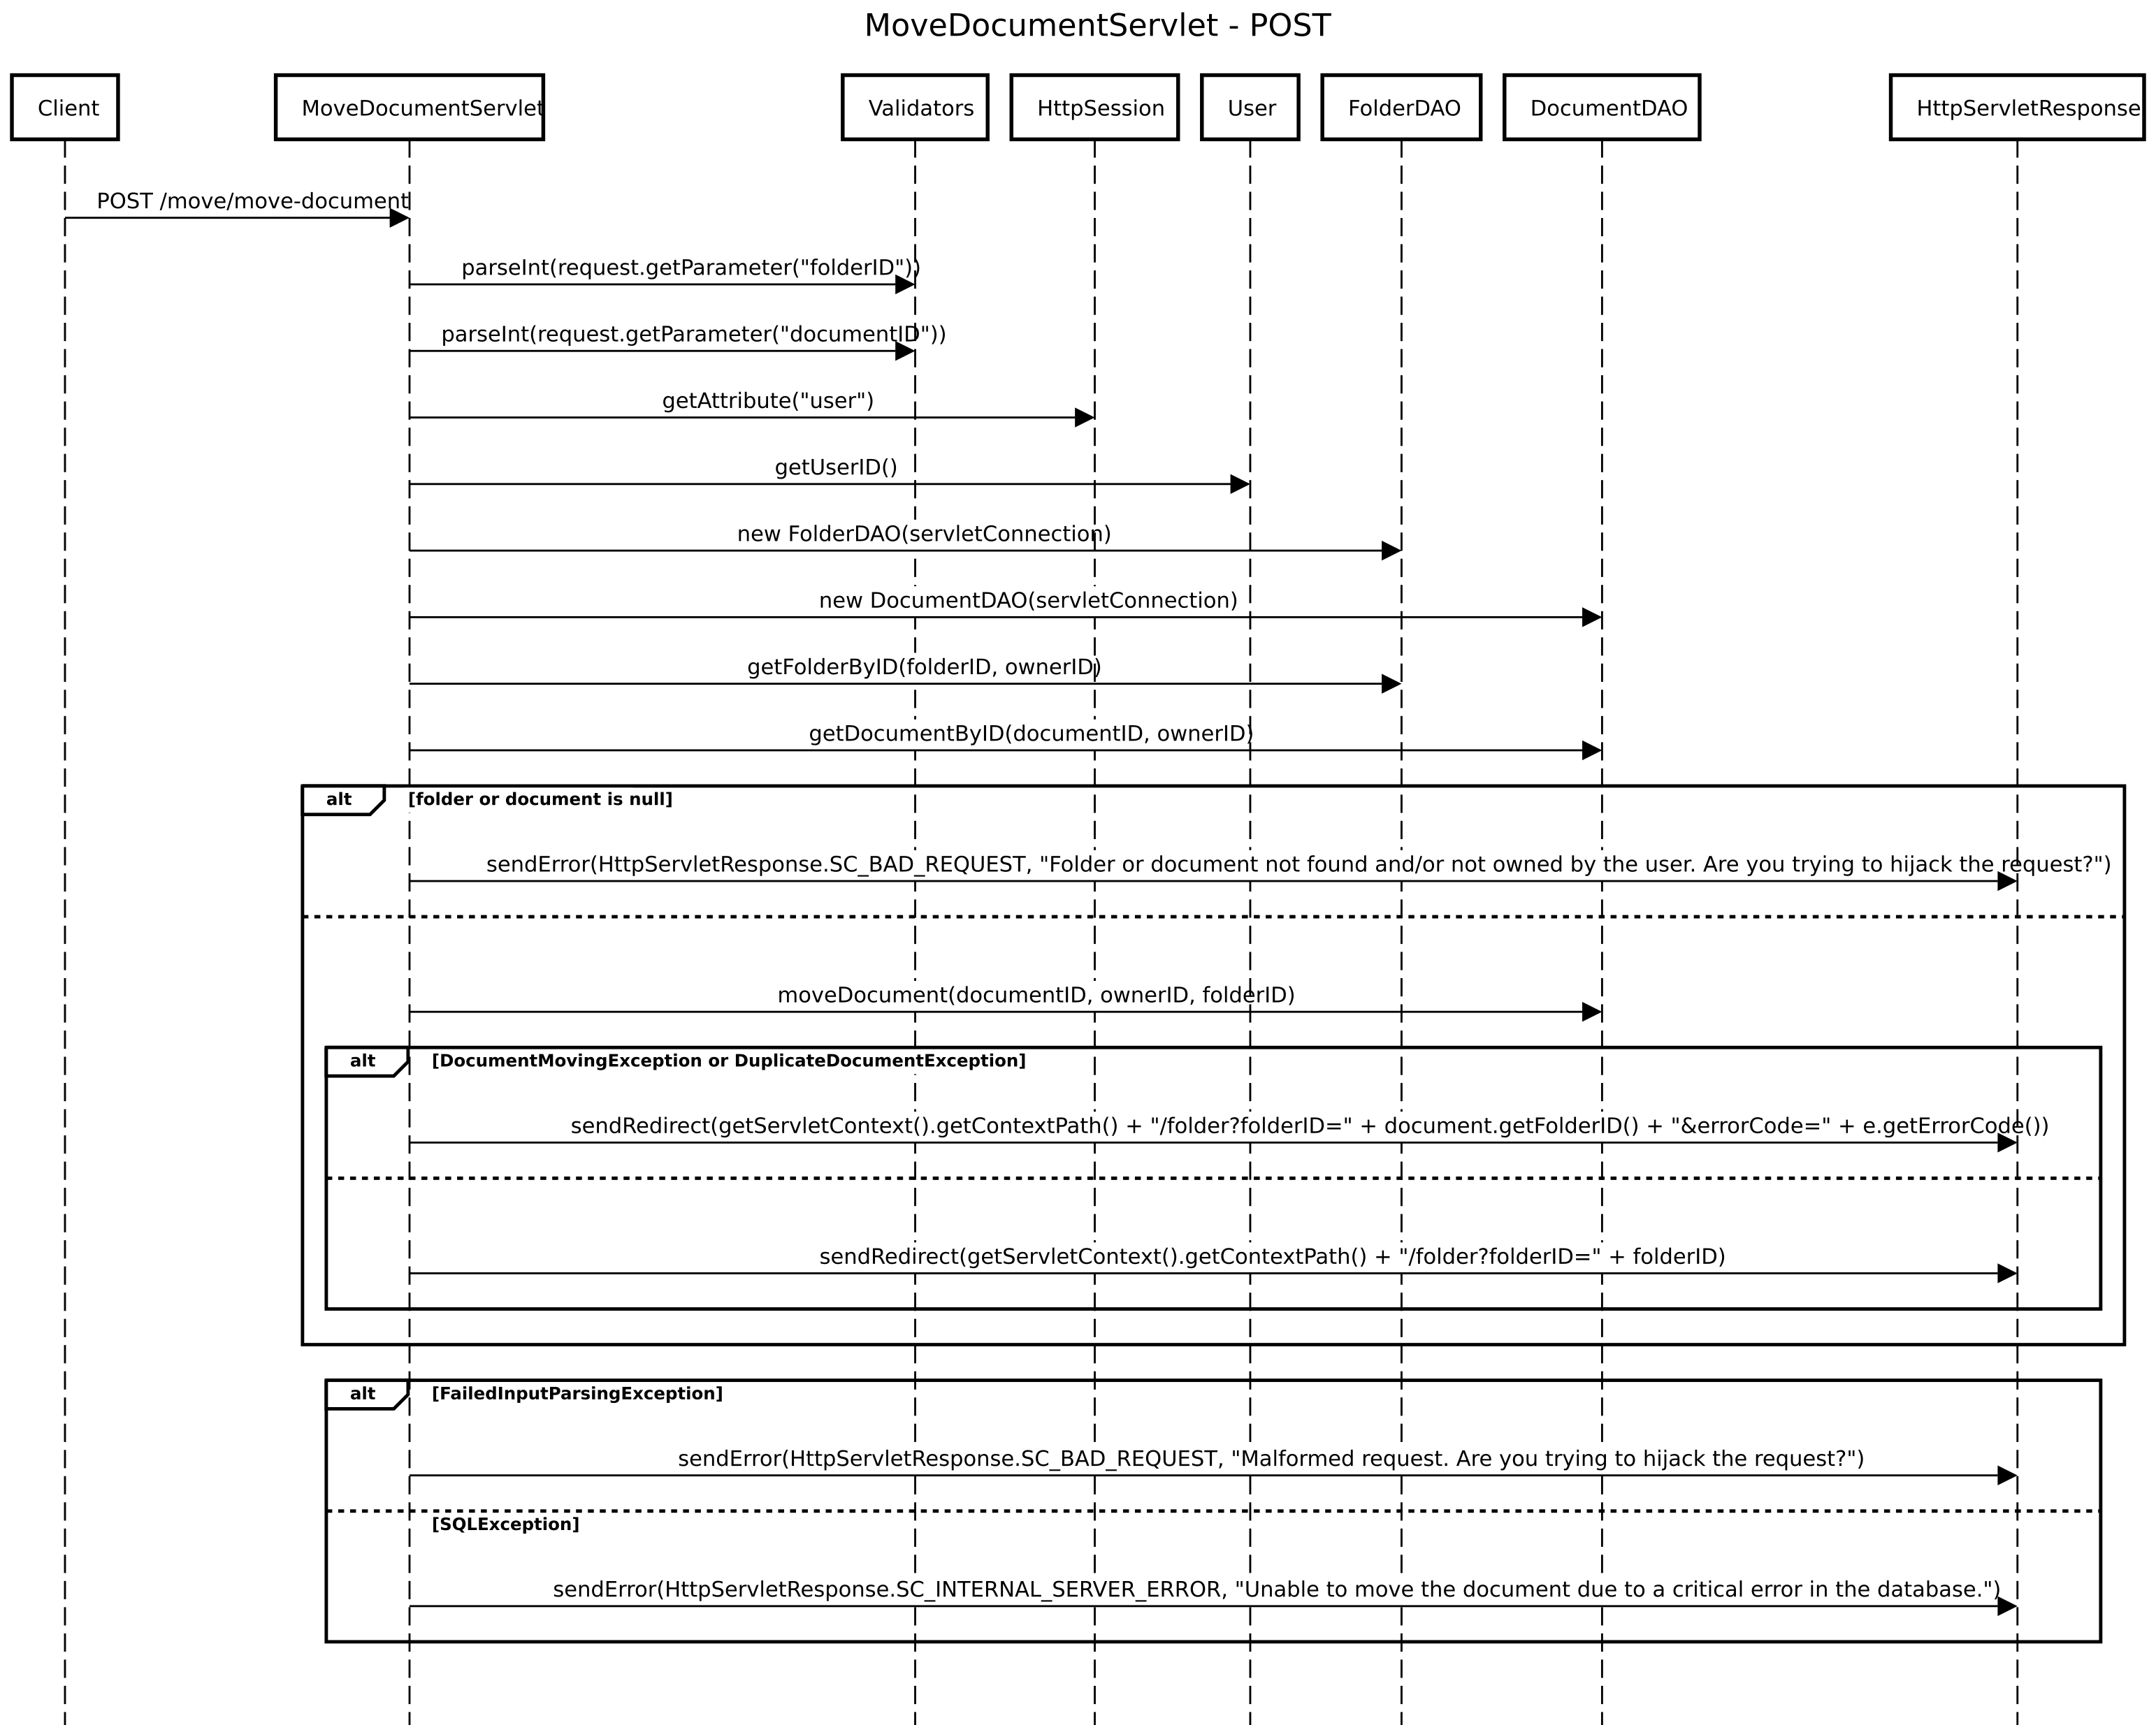
\includegraphics[width=\dimexpr 0.95\paperwidth\relax, height=\dimexpr 0.90\paperheight\relax,
            keepaspectratio]{Resources/SequenceDiagrams/images/MoveDocumentServlet - POST.png}
    \end{figure}
\end{frame}

\begin{frame}
    \begin{figure}
        \centering
        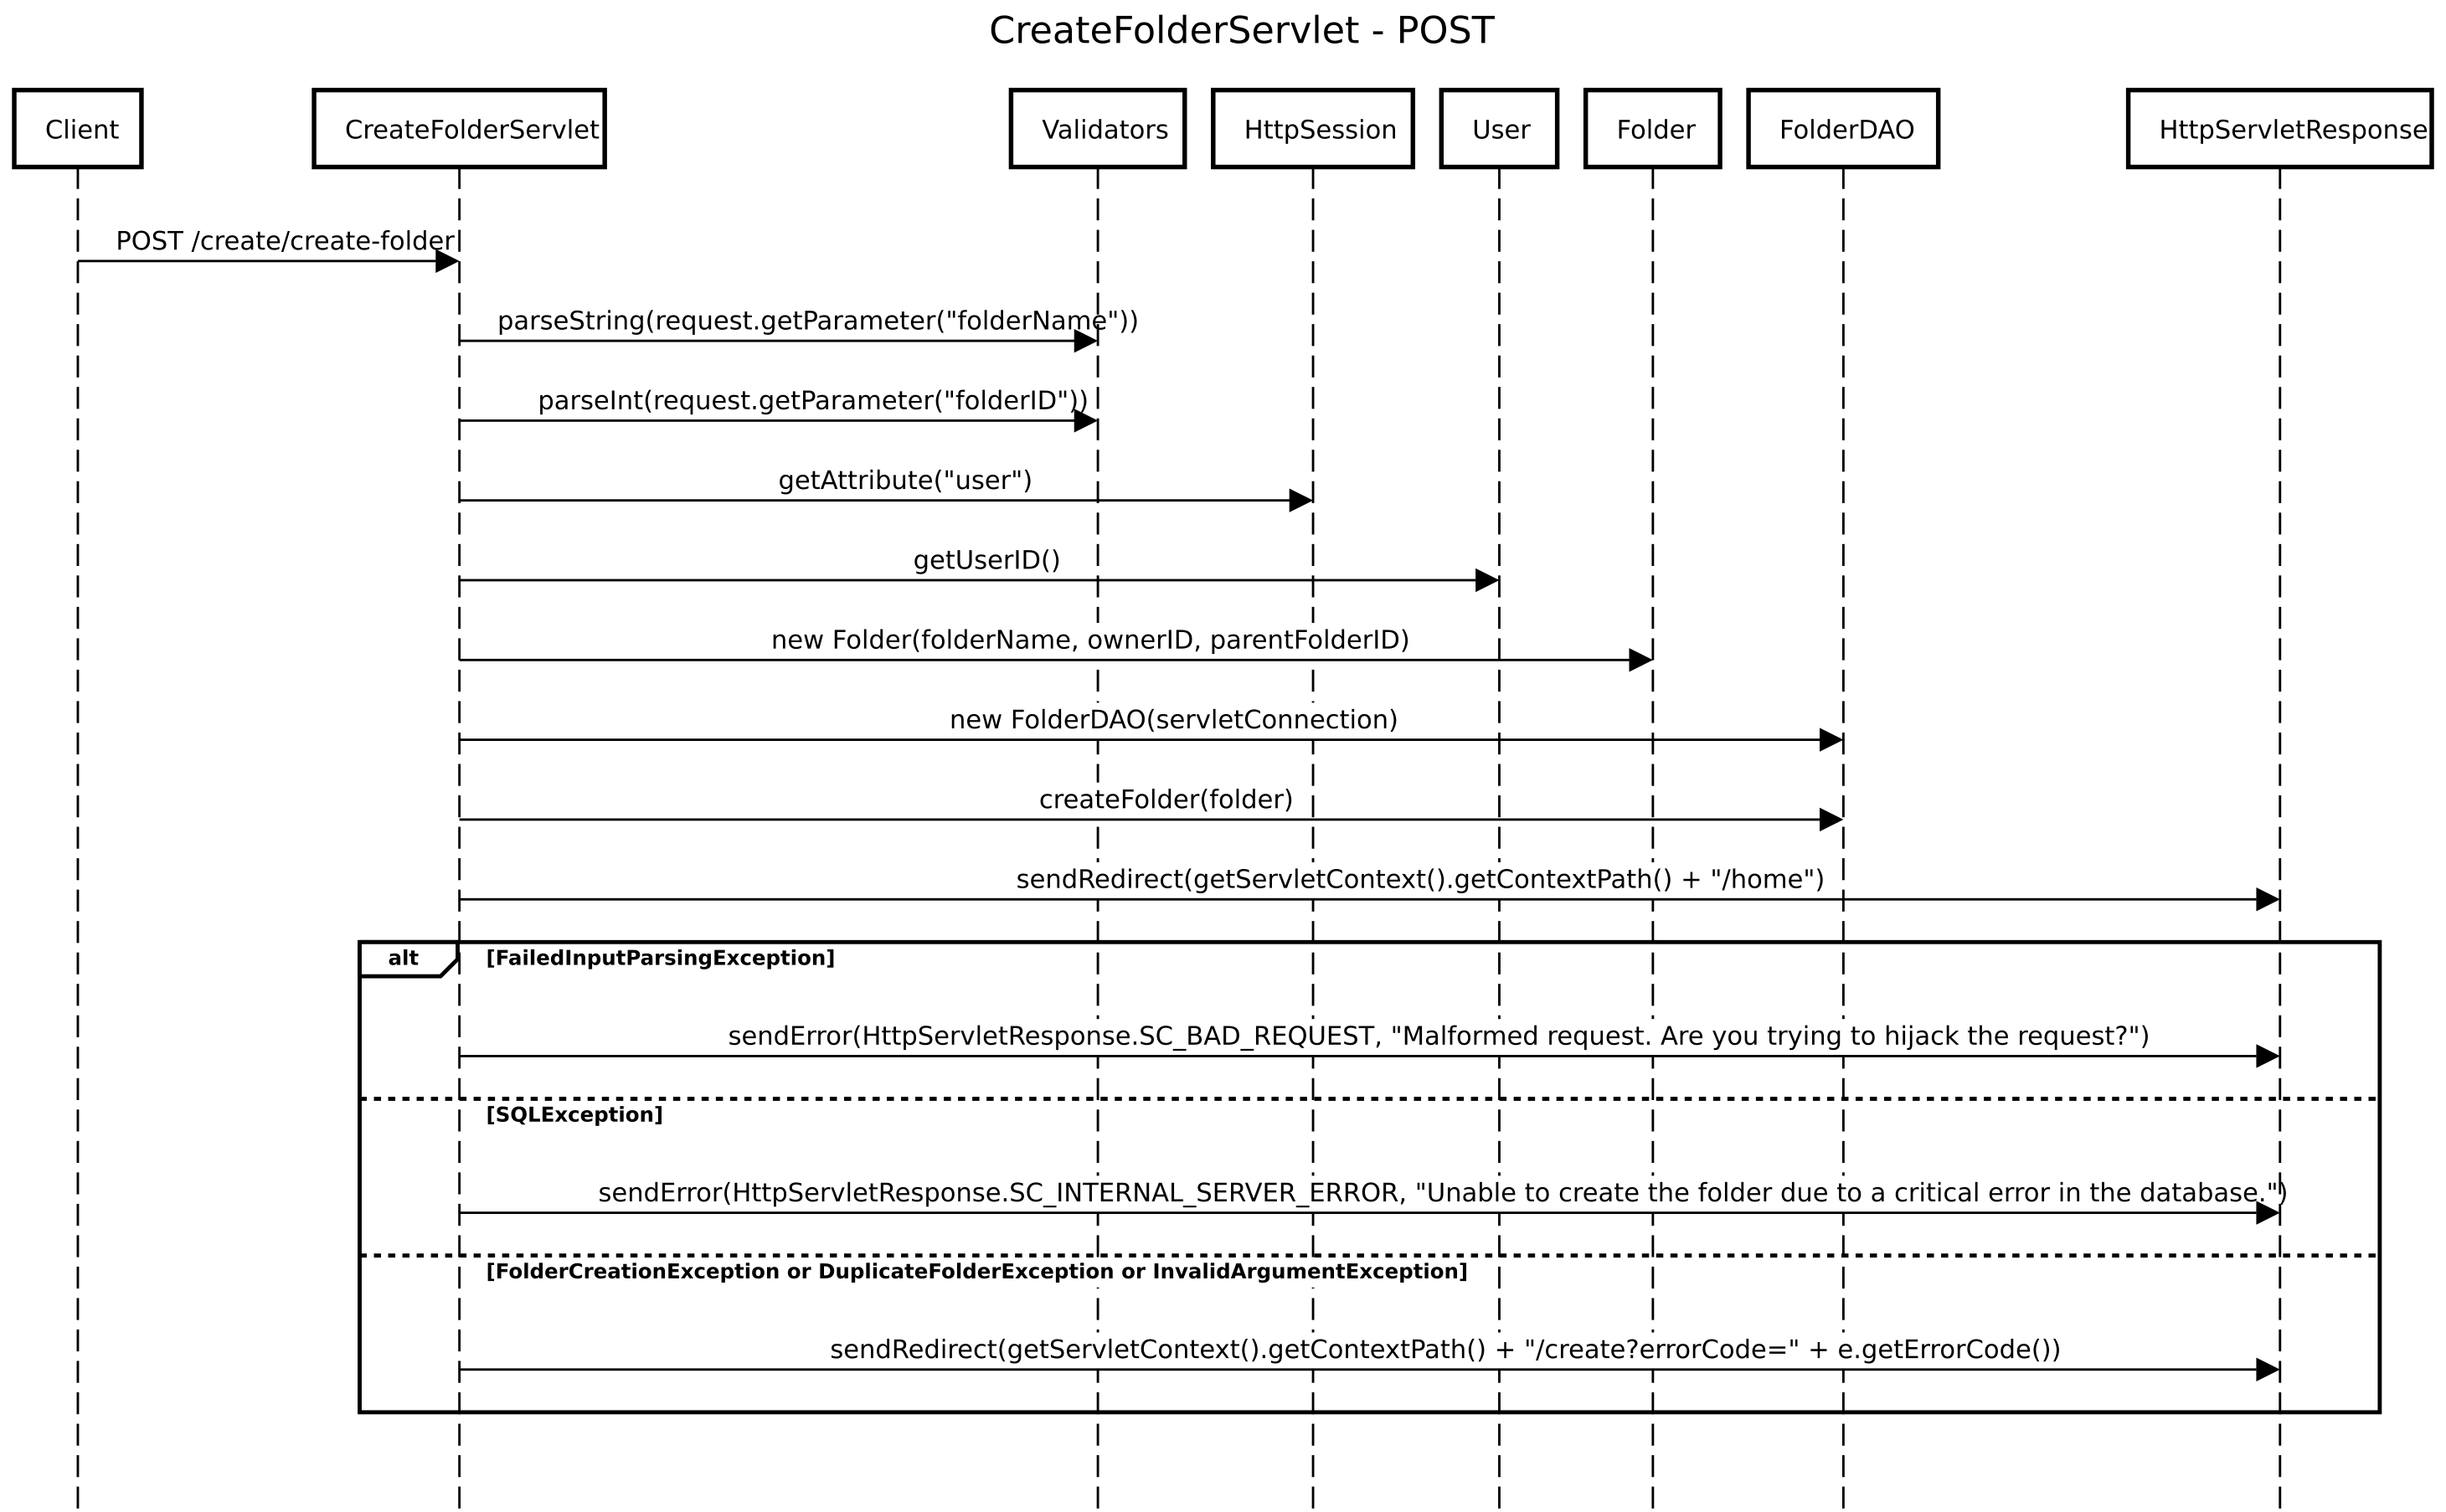
\includegraphics[width=\dimexpr 0.95\paperwidth\relax, height=\dimexpr 0.90\paperheight\relax,
            keepaspectratio]{Resources/SequenceDiagrams/images/CreateFolderServlet - POST.png}
    \end{figure}
\end{frame}

\begin{frame}
    \begin{figure}
        \centering
        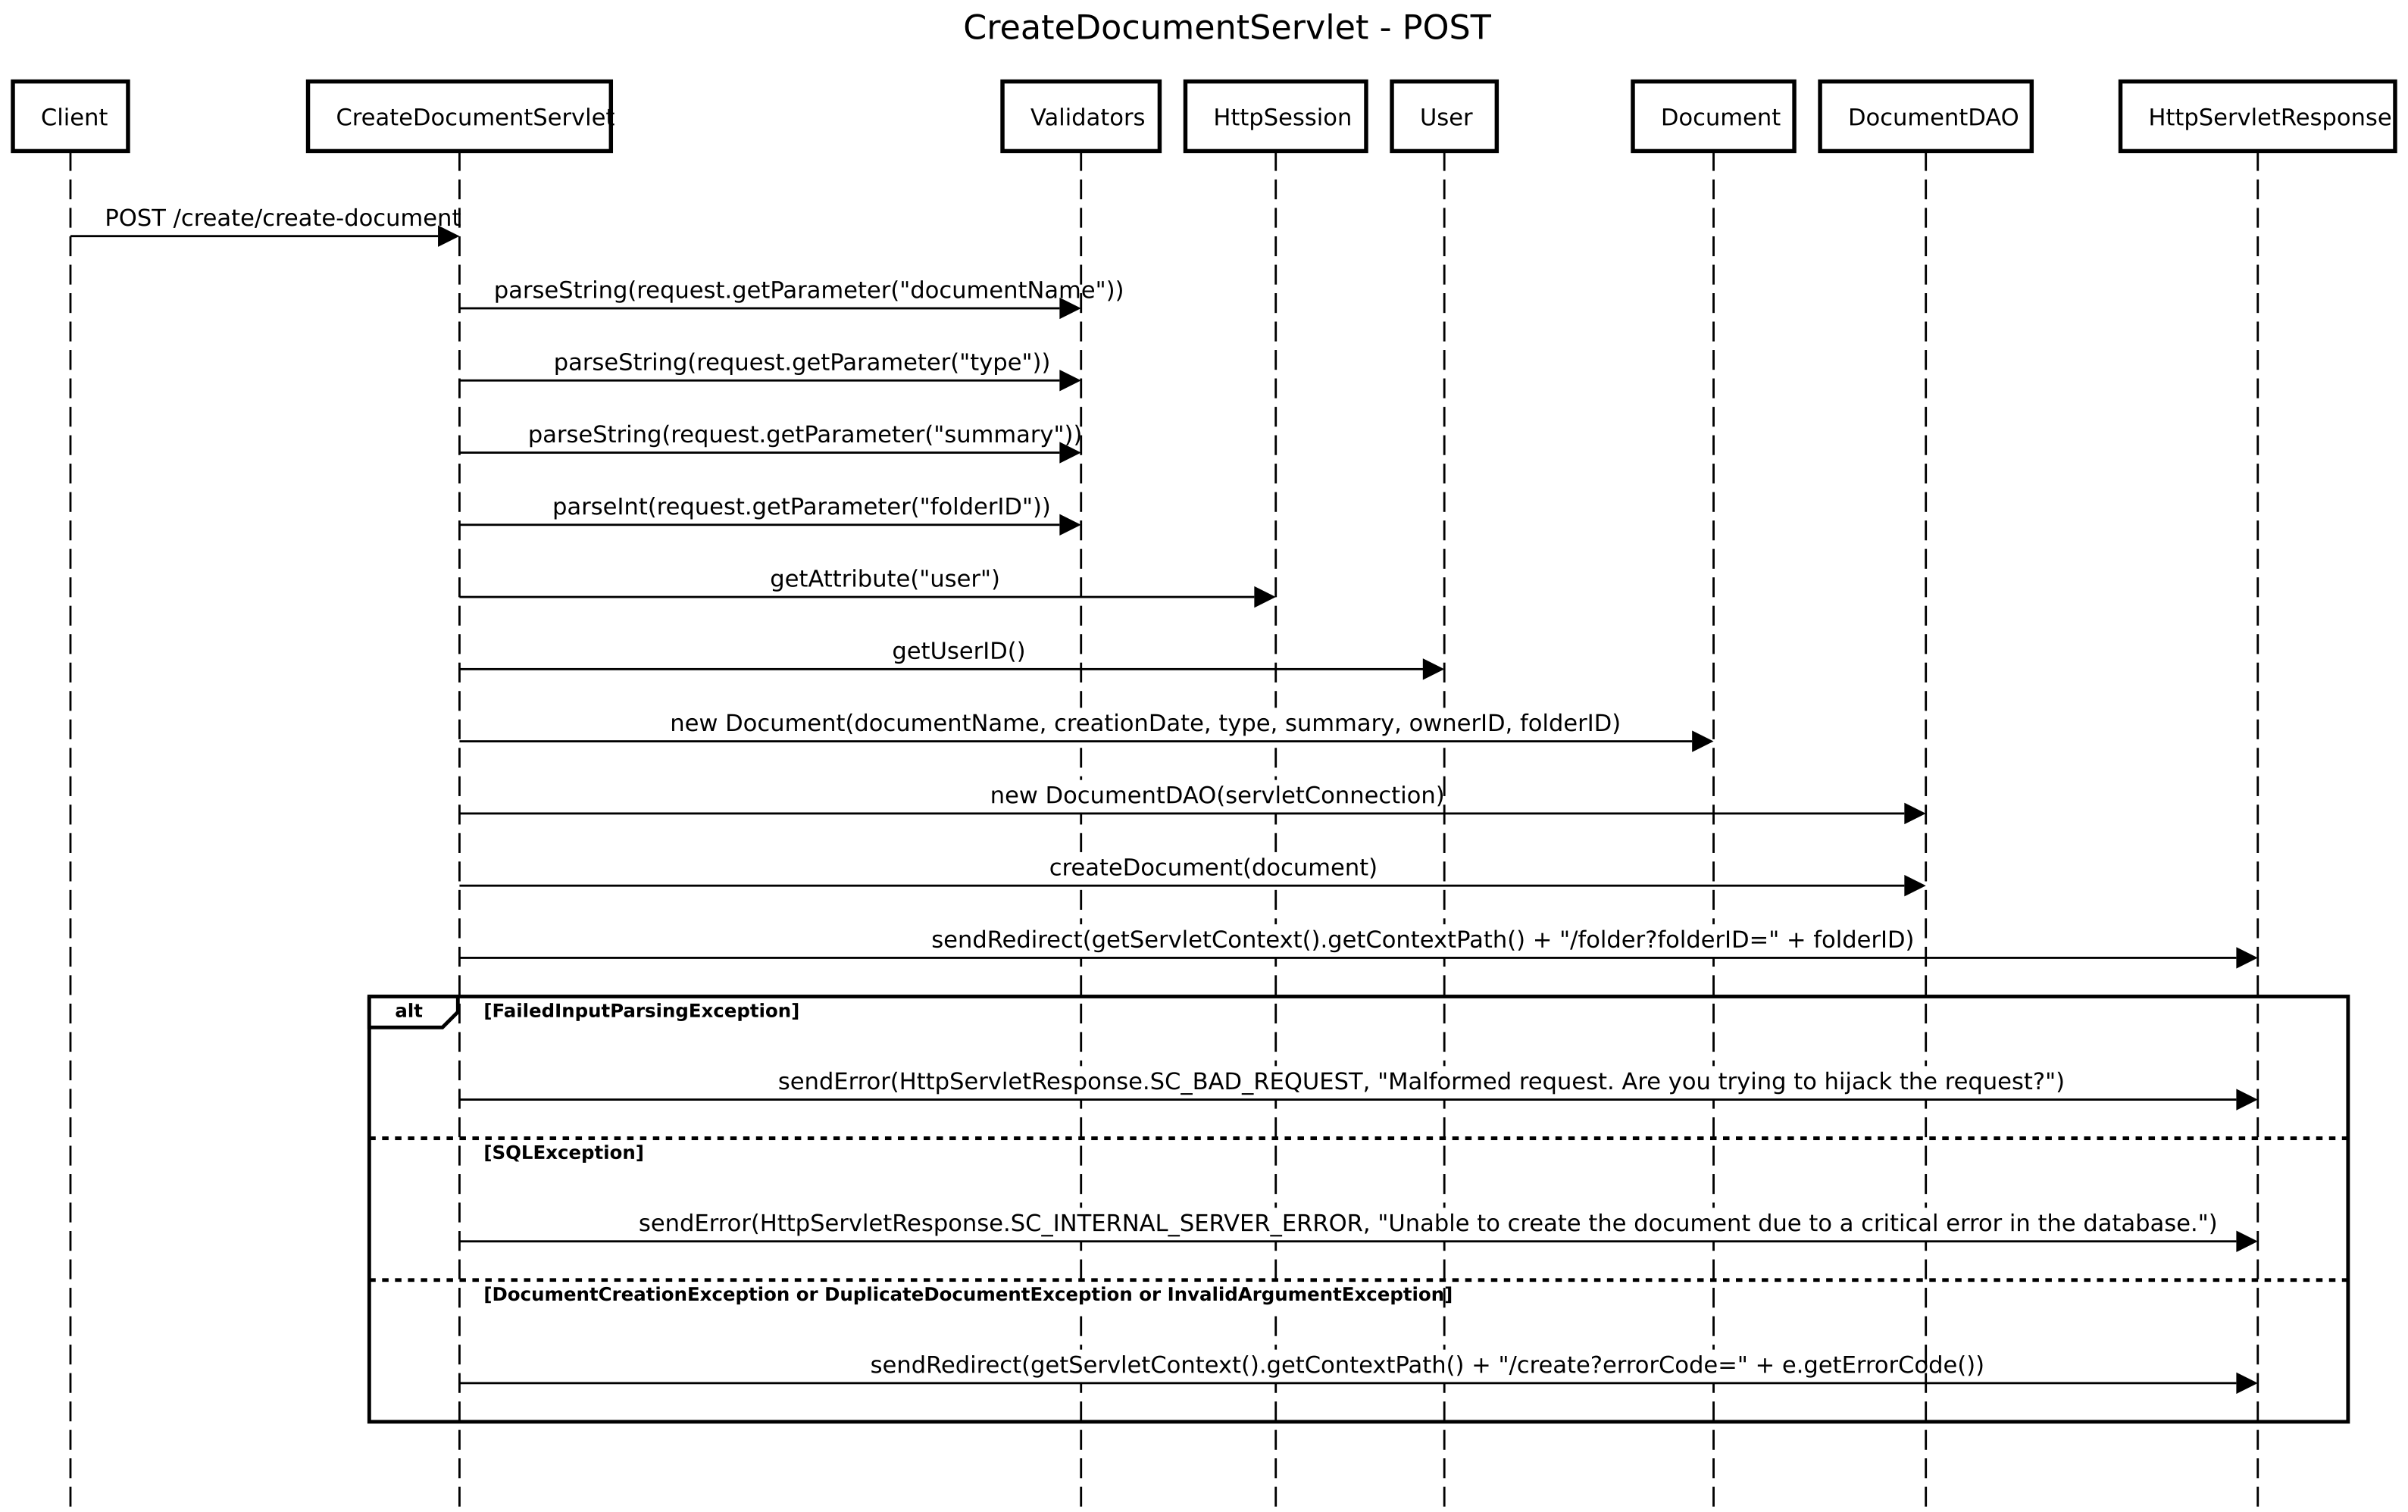
\includegraphics[width=\dimexpr 0.95\paperwidth\relax, height=\dimexpr 0.90\paperheight\relax,
            keepaspectratio]{Resources/SequenceDiagrams/images/CreateDocumentServlet - POST.png}
    \end{figure}
\end{frame}

\begin{frame}
    \begin{figure}
        \centering
        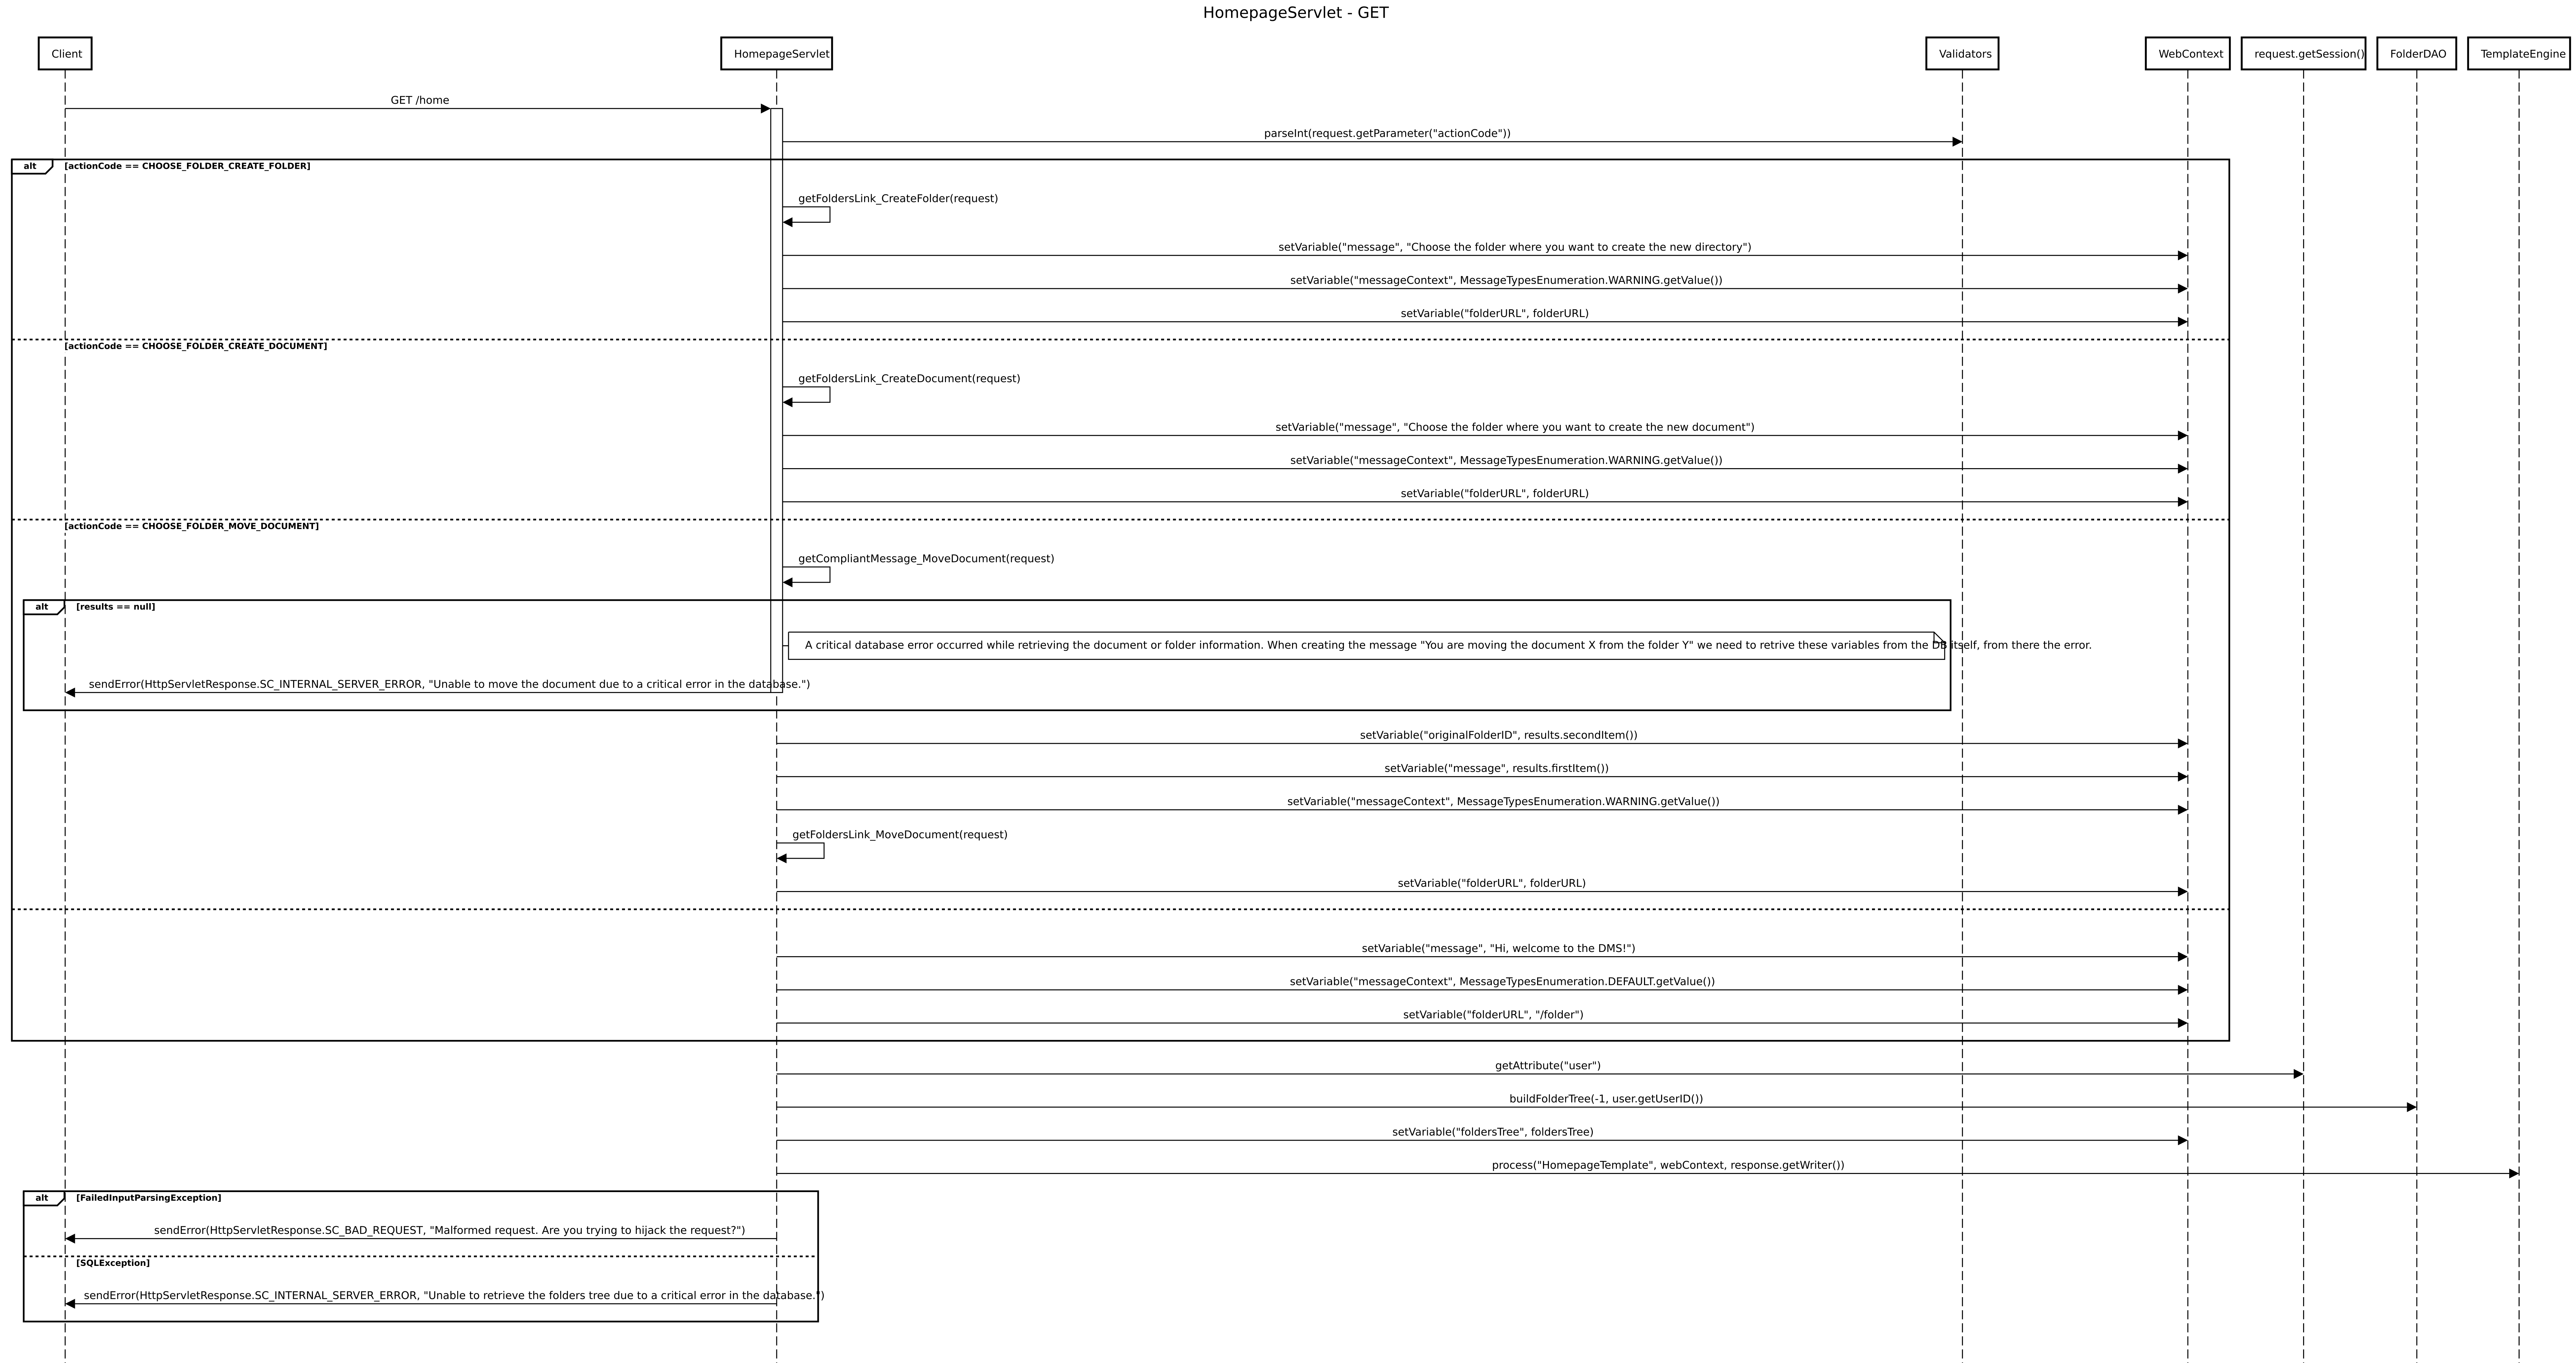
\includegraphics[width=\dimexpr 0.95\paperwidth\relax, height=\dimexpr 0.90\paperheight\relax,
            keepaspectratio]{Resources/SequenceDiagrams/images/HomepageServlet - GET.png}
    \end{figure}
\end{frame}

\end{document}